\documentclass[10pt,journal,compsoc]{IEEEtran}
\IEEEoverridecommandlockouts

% -------------------- Essential Packages --------------------
\usepackage[cmex10]{amsmath}
\usepackage{amssymb,amsfonts,amsthm,mathtools,bm}
\usepackage{algorithm}
\usepackage{algorithmic}
\usepackage{graphicx}
\usepackage{textcomp}
\usepackage{xcolor}
\ifCLASSOPTIONcompsoc
  \usepackage[nocompress]{cite}
\else
  \usepackage{cite}
\fi
\usepackage{url}
\usepackage{booktabs}
\usepackage{multirow}
\usepackage{array}
\usepackage{tikz}
\usepackage{pgfplots}
\pgfplotsset{compat=1.17}
\usetikzlibrary{positioning,arrows,shapes,calc}
\usepackage{soul}
\usepackage{enumitem}
\usepackage{listings}
\usepackage{microtype}
\usepackage[caption=false,font=footnotesize]{subfig}
\usepackage[hidelinks]{hyperref}

\usepackage[nameinlink,capitalise,noabbrev]{cleveref}

\usepackage{tabularx}

% -------------------- Custom Commands --------------------
\newcommand{\R}{\mathbb{R}}
\newcommand{\E}{\mathbb{E}}
\newcommand{\N}{\mathcal{N}}
\newcommand{\F}{\mathcal{F}}
\newcommand{\G}{\mathcal{G}}
\newcommand{\D}{\mathcal{D}}
\newcommand{\A}{\mathcal{A}}
\newcommand{\X}{\mathcal{X}}
\newcommand{\Y}{\mathcal{Y}}
\newcommand{\Z}{\mathcal{Z}}
\newcommand{\s}{\mathcal{S}}
\newcommand{\Tcal}{\mathcal{T}}
\newcommand{\Kcal}{\mathcal{K}}
\newcommand{\Mcal}{\mathcal{M}}
\newcommand{\Q}{\mathcal{Q}}
\newcommand{\U}{\mathcal{U}}
\newcommand{\V}{\mathcal{V}}
\newcommand{\W}{\mathcal{W}}
\newcommand{\h}{\mathcal{H}}
\newcommand{\softplus}{\operatorname{softplus}}
\newcommand{\Softmax}{\operatorname{Softmax}}

\DeclareMathOperator*{\argmin}{arg\,min}
\DeclareMathOperator*{\argmax}{arg\,max}
\DeclareMathOperator{\Tr}{Tr}
\DeclareMathOperator{\diag}{diag}
\DeclareMathOperator{\rank}{rank}
\DeclareMathOperator{\vecop}{vec}
\DeclareMathOperator{\prox}{prox}
\DeclareMathOperator{\KL}{KL}
\DeclareMathOperator{\ELBO}{ELBO}

% -------------------- Theorem Environments --------------------
\newtheorem{theorem}{Theorem}
\newtheorem{lemma}[theorem]{Lemma}
\newtheorem{proposition}[theorem]{Proposition}
\newtheorem{corollary}[theorem]{Corollary}
\newtheorem{definition}{Definition}
\newtheorem{assumption}{Assumption}
\newtheorem{remark}{Remark}

% Tighten spacing around floats
\setlength{\textfloatsep}{5pt}% space between text and floats
\setlength{\floatsep}{5pt}% space between two floats
\setlength{\intextsep}{5pt}% space above and below in-text floats
\setlength{\skip\footins}{8pt}% space above footnotes



% -------------------- Title & Authors --------------------
\title{Temporal Adaptive Neural Ordinary Differential Equations with Deep Spatio-Temporal Point Processes for Real-Time Network Intrusion Detection}

\author{%
Roger~Nick~Anaedevha,~\IEEEmembership{Student Member,~IEEE}\IEEEauthorrefmark{1},
Alexander~Gennadevich~Trofimov\IEEEauthorrefmark{1},
and~Yuri~Vladimirovich~Borodachev\IEEEauthorrefmark{2}\\
\IEEEauthorrefmark{1}National Research Nuclear University MEPhI (Moscow Engineering Physics Institute), Moscow 115409, Russia\\
\IEEEauthorrefmark{2}Artificial Intelligence Research Center, National Research Nuclear University MEPhI, Moscow 115409, Russia\\
Corresponding author: \href{mailto:ar006@campus.mephi.ru}{ar006@campus.mephi.ru}
}
% -------------------- Document --------------------
\begin{document}
\maketitle

\begin{abstract}
Network attacks exploit complex temporal dependencies spanning microseconds to months, requiring unified modelling of continuous system dynamics and discrete event occurrences. This paper introduces a framework integrating Temporal Adaptive Batch Normalization Neural Ordinary Differential Equations (TA-BN-ODE) with Deep Spatio-Temporal Point Processes (DSTPP) for real-time adaptive intrusion detection. We present five fundamental contributions validated on the Integrated Cloud Security 3Datasets comprising 18.9 million security records across container orchestration, IoT/IIoT networks, and enterprise security operations. First, we develop security-specific TA-BN-ODE architectures achieving 97.3\% accuracy with 60--90\% parameter reduction through continuous-depth adaptation and stability guarantees. Second, we introduce transformer-enhanced marked temporal point processes with log-barrier optimization reducing complexity from cubic to quadratic scaling while capturing multi-scale temporal patterns. Third, we present structured variational Bayesian inference providing calibrated uncertainty quantification with 91.7\% coverage probability and PAC-Bayesian generalisation  bounds. Fourth, we demonstrate Large Language Model integration achieving 87.6\% F1-score on zero-shot detection of novel attacks. Fifth, we provide theoretical convergence guarantees for online learning under concept drift with differential privacy preservation. Our framework processes 12.3 million events per second with sub-100ms latency, achieving 99.4\% accuracy on container security, 98.6\% on IoT networks, and 92.7\% F1-score on enterprise incident triage. Comprehensive evaluation on standard benchmarks (CIC-IDS2018, UNSW-NB15, CIC-IoT-2023) and comparison with continuous-time models demonstrate state-of-the-art performance with 82\% parameter reduction. Cross-domain validation on speech processing and healthcare monitoring confirms broad applicability beyond network security.
\end{abstract}

\vspace{-0.2cm}

\begin{IEEEkeywords}
Neural ordinary differential equations, temporal point processes, real-time detection, Bayesian inference, transformer models, continuous-depth networks, IoT security, uncertainty quantification, intrusion detection systems
\end{IEEEkeywords}

\IEEEpeerreviewmaketitle

% =========================================================
\vspace{-0.2cm}
\section{Introduction}
\label{sec:introduction}

Network intrusion detection systems face escalating complexity as adversaries exploit temporal dependencies across multiple time scales while the proliferation of IoT devices creates billions of vulnerable endpoints. Industry reports indicate that 67\% of organisations encountered temporal-based attacks in 2024~\cite{verizon2024dbir}, with detection delays exceeding 200 days and average breach costs of \$4.35 million~\cite{ibm2024breach}. These sophisticated attacks operate across eight orders of magnitude in time scales, from microsecond-level timing attacks to month-long Advanced Persistent Threat campaigns, fundamentally challenging discrete-time detection approaches that sample at fixed intervals.

Consider a concrete example illustrating the limitations of discrete sampling: An Advanced Persistent Threat conducts reconnaissance by probing vulnerable ports at carefully randomized intervals spanning 10 seconds to 60 minutes, specifically designed to evade fixed-window detectors. Traditional systems sampling every minute miss 73\% of such probes, while continuous models tracking instantaneous event intensity $\lambda(t)$ detect anomalous inter-arrival patterns regardless of probe timing. This motivates our continuous-discrete hybrid approach that jointly models smooth system state evolution through Neural ODEs and irregular event occurrences through temporal point processes.

\vspace{-0.2cm}
\subsection{Technical Challenges in Temporal Security modelling}

Coupling continuous dynamics with discrete temporal modelling for network security poses several fundamental challenges. First, batch normalization designed for discrete layers with fixed statistics proves incompatible with Neural ODEs requiring time-dependent normalization—without adaptation, gradients explode and deep ODE stacks become unstable. Second, real-time monitoring demands processing millions of events per second with sub-millisecond latency, but adaptive ODE solvers and self-attention mechanisms scale poorly, with standard transformers exhibiting $O(n^2)$ complexity. Third, security analysts need calibrated confidence intervals to triage alerts effectively, yet existing ODE and point process approaches provide only point estimates with poor calibration under distribution shift. Fourth, models must adapt online to concept drift from software updates and evolving attacks~\cite{gama2014survey} without costly retraining while maintaining theoretical convergence guarantees. Finally, effective frameworks must generalize across container, IoT, and enterprise networks without brittle domain-specific tuning.

\vspace{-0.2cm}
\subsection{Recent Algorithmic Breakthroughs}

Two recent algorithmic advances enable our unified framework. Temporal Adaptive Batch Normalization, introduced at NeurIPS 2024~\cite{salvi2024tabn}, extends batch normalization to continuous time by modelling normalization statistics as functions of integration time, resolving the incompatibility between discrete normalization and continuous dynamics. This breakthrough enables stable stacking of Neural ODE layers achieving state-of-the-art continuous-time modelling. Concurrently, integrating large language models with temporal point processes demonstrates that prompt-based adaptation and chain-of-thought reasoning enable foundation models to perform zero-shot temporal event prediction~\cite{xue2024prompted,wei2022chain}, signaling a paradigm shift from supervised signature matching to semantic understanding of attack strategies.

\vspace{-0.2cm}
\subsection{Research Contributions}

This paper addresses these fundamental challenges through a unified framework achieving both theoretical advances and practical breakthroughs in network intrusion detection. Our contributions span architectural innovations, algorithmic developments, theoretical analysis, and comprehensive empirical validation on diverse security datasets.

Contribution 1: Security-Specific TA-BN-ODE Architectures. We develop Temporal Adaptive Batch Normalization Neural ODE architectures achieving 97.3\% accuracy with 60--90\% fewer parameters than discrete networks. Our continuous-depth adaptation mechanism allocates computational resources proportional to input complexity, increasing integration time for complex attack patterns while processing benign traffic efficiently. Stability analysis through Lyapunov theory ensures bounded gradients preventing exploding gradient problems during adjoint computation.

Contribution 2: Multi-Scale Deep Spatio-Temporal Point Processes. We introduce transformer-enhanced marked temporal point processes with logarithmic barrier optimization reducing computational complexity from $O(n^3)$ to $O(n^2)$ in sequence length. The multi-scale architecture captures patterns across eight orders of magnitude—from microsecond timing attacks to month-long APT campaigns—through hierarchical decomposition with learned time constants enabling simultaneous modelling of rapid bursts, diurnal patterns, and long-term trends.

Contribution 3: Structured Variational Bayesian Inference. We present structured variational Bayesian inference with mean-field approximation and strategic dependency structure achieving 91.7\% coverage probability for prediction intervals. The uncertainty quantification enables calibrated confidence estimates reducing false positive investigation time by 43\% in operational deployments through reliable confidence-based filtering. PAC-Bayesian generalisation  bounds provide finite-sample risk guarantees justifying our structured posterior choice.

Contribution 4: LLM-Integrated Zero-Shot Detection. We demonstrate Large Language Model integration through carefully designed prompt engineering achieving 87.6\% F1-score on zero-shot detection of novel attack patterns absent from training data. Temporal reasoning prompts enable language models to analyze attack sequences, identify anomalous behaviours, and generate semantic explanations, enabling proactive defence through transfer of general security knowledge rather than reactive detection based solely on historical signatures.

Contribution 5: Online Learning with Convergence Guarantees. We provide theoretical convergence guarantees for online learning under concept drift with formal differential privacy preservation. Our analysis proves adaptive learning rates achieve sublinear regret bounds even with distribution shift, establishing conditions under which the system provably adapts to evolving attack landscapes. Differential privacy analysis ensures model updates do not leak sensitive information about individual flows or user behaviours.

\vspace{-0.2cm}
\subsection{Comprehensive Experimental Validation}

We provide extensive validation on multiple datasets demonstrating broad applicability. The Integrated Cloud Security 3Datasets (ICS3D) comprises 18.9 million security records across 8.4 gigabytes spanning three critical domains: container orchestration security (697,289 flows from Kubernetes clusters), IoT/IIoT security (4 million records from seven-layer testbed), and enterprise SOC incidents (1 million alerts from 6,100 organisation s with MITRE ATT\&CK annotations). Additionally, we evaluate on three standard benchmarks—CIC-IDS2018, UNSW-NB15, and CIC-IoT-2023—enabling direct comparison with published baselines. Comparison with our recent multimodal transformer work~\cite{anaedevha2026stochastic} and continuous-time models (Neural CDE, GRU-ODE) demonstrates superior parameter efficiency and accuracy. Cross-domain validation on speech event detection (LibriSpeech) and healthcare monitoring (MIMIC-III, eICU) confirms that our continuous-discrete hybrid modelling approach extends beyond network security.

\vspace{-0.2cm}
\subsection{organisation }

This paper presents a comprehensive treatment balancing mathematical rigor with practical implementation. Section~\ref{sec:related} reviews related work across Neural ODEs, temporal point processes, intrusion detection systems, Bayesian inference, and recent security-specific models. Section~\ref{sec:framework} establishes mathematical foundations and problem formulation. Section~\ref{sec:tabn_ode} develops TA-BN-ODE architectures with stability analysis and Algorithm~\ref{alg:tabn_ode_forward}. Section~\ref{sec:point_processes} introduces deep spatio-temporal point processes with complexity reduction. Section~\ref{sec:bayesian} presents structured variational inference with PAC-Bayesian bounds. Section~\ref{sec:llm_integration} describes LLM integration for zero-shot detection. Section~\ref{sec:datasets} details dataset characteristics and preprocessing. Section~\ref{sec:experiments} provides comprehensive experimental evaluation including standard benchmarks and continuous-time baseline comparisons. Section~\ref{sec:discussion} discusses implications, limitations, and future directions. Section~\ref{sec:conclusion} concludes with summary and broader impact. Supplementary materials provide extended proofs (Theorems 1-5), per-attack performance analysis, complete hyperparameter configurations, and additional cross-domain results.

% =========================================================
\vspace{-0.2cm}
\section{Related Work}
\label{sec:related}

This section reviews prior research across interconnected areas foundational to our framework, emphasizing recent breakthroughs while identifying limitations our work addresses.

\vspace{-0.2cm}
\subsection{Neural Ordinary Differential Equations}

Neural ODEs, introduced by Chen et al.~\cite{chen2018neural}, parameterise network dynamics as continuous-time ODEs $\frac{dh}{dt} = f_\theta(h, t)$, enabling memory-efficient backpropagation through adjoint methods~\cite{pontryagin1962mathematical}. Subsequent advances include state augmentation for enhanced expressiveness~\cite{dupont2019augmented}, optimal transport formulations~\cite{onken2021ot}, and stability analyses through Lyapunov theory~\cite{lu2018beyond}. Recent work explores adversarial robustness through orthogonal ODEs~\cite{purohit2024ortho} and closed-form continuous networks~\cite{hasani2022liquid}. However, cybersecurity applications remain largely unexplored despite their natural fit for modelling temporal attack evolution.

A critical obstacle has been the incompatibility between batch normalization—designed for discrete layers with fixed statistics—and continuous dynamics. Standard batch normalization applies time-independent normalization causing gradient explosion in deep ODE stacks. Salvi et al.~\cite{salvi2024tabn} recently resolved this through Temporal Adaptive Batch Normalization, parameterizing normalization statistics as functions of integration time. We extend this breakthrough to security applications, developing stability guarantees and multi-scale architectures tailored for intrusion detection.

\vspace{-0.2cm}
\subsection{Continuous-Time Models for Temporal Data}

Beyond Neural ODEs, several continuous-time approaches model irregular temporal data. Neural Controlled Differential Equations (Neural CDEs)~\cite{kidger2020neural} use continuous controls for time-series with missing data, achieving strong interpolation performance. GRU-ODE~\cite{de2019gru} combines recurrent structures with ODE dynamics, while Latent ODEs~\cite{rubanova2019latent} learn latent representations through variational autoencoders. Continuous Normalizing Flows~\cite{grathwohl2018ffjord} provide tractable density estimation via change-of-variables. However, these models focus primarily on interpolation and forecasting rather than event detection, lack explicit uncertainty quantification, and do not incorporate discrete event intensities through point processes—critical for security applications where event timing carries strong signal.

\vspace{-0.2cm}
\subsection{Temporal Point Processes}

Temporal point processes model irregular event sequences through conditional intensity functions $\lambda^*(t)$~\cite{daley2003introduction}. Classical Hawkes processes~\cite{hawkes1971spectra} capture self-excitation where past events increase future occurrence probability. Recent neural variants leverage recurrent networks~\cite{du2016recurrent} and transformers~\cite{zuo2020transformer,zhang2020selfatt} for expressive intensity modelling. Shchur et al.~\cite{shchur2021neural} propose intensity-free learning avoiding numerical integration challenges.

In intrusion detection, Gao et al.~\cite{gao2024hplstm} combine Hawkes processes with LSTMs (HP-LSTM) but remain discrete-time and lack principled uncertainty quantification. Our framework advances beyond HP-LSTM through: (1) continuous dynamics via Neural ODEs rather than discrete LSTM, (2) multi-scale temporal encoding spanning microseconds to months, (3) log-barrier optimization reducing complexity from cubic to quadratic, and (4) rigorous Bayesian uncertainty quantification with calibration guarantees.

\vspace{-0.2cm}
\subsection{Network Intrusion Detection Systems}

Traditional intrusion detection relies on signature matching and rule-based systems~\cite{scarfone2007guide}, limited to known attacks. Machine learning approaches including SVMs~\cite{mukkamala2002intrusion}, random forests~\cite{panda2011network}, and ensemble methods~\cite{gaikwad2014intrusion} improve generalisation  but struggle with temporal dependencies. Deep learning advances include CNNs for spatial feature extraction~\cite{vinayakumar2017applying}, LSTMs for sequential modelling~\cite{kim2016lstm}, and attention mechanisms~\cite{vaswani2017attention}. Transformer-based systems~\cite{jiang2020transformer} achieve strong performance on spatial features but discretize time, missing critical timing information.

Recent security-specific neural models include Graph Neural Networks for network topology~\cite{kipf2017semi,jiang2019graph}, adversarially robust detectors~\cite{corona2019adversarial}, and federated learning for privacy-preserving training~\cite{mothukuri2021federated}. However, none integrate continuous dynamics, point processes, Bayesian uncertainty, and LLM-based zero-shot detection in a unified framework optimised for multi-scale temporal attack patterns.

\vspace{-0.2cm}
\subsection{Comparison with Recent Multimodal Work}

Our recent work~\cite{anaedevha2026stochastic} introduced a Stochastic Multimodal Transformer with Uncertainty Quantification achieving strong results on standard benchmarks (CIC-IDS2018: 98.2\%, UNSW-NB15: 97.4\%, CIC-IoT-2023: 98.8\%). While that approach excels at multi-modal feature fusion through cross-attention and provides uncertainty via Monte Carlo dropout, it operates in discrete time with fixed-depth transformers requiring 15.7M parameters. The current work advances beyond our prior contribution through: (1) continuous-depth adaptation via Neural ODEs reducing parameters by 82\% (2.3M vs 15.7M), (2) explicit temporal point process modelling capturing event timing information, (3) multi-scale architecture spanning eight orders of magnitude in time scales, (4) structured variational Bayesian inference with PAC-theoretical guarantees rather than empirical dropout approximation, and (5) LLM integration for semantic zero-shot detection. Table~\ref{tab:comparison_multimodal} provides detailed comparison demonstrating complementary strengths—multimodal fusion for feature-rich scenarios versus continuous temporal modelling for time-critical detection.

\begin{table}[!t]
\centering
\small
\setlength{\tabcolsep}{3pt}
\caption{Side-by-side comparison of continuous-time TA-BN-ODE vs. discrete multimodal transformer for IDS.}
\label{tab:comparison_multimodal}
\newcolumntype{Y}{>{\raggedright\arraybackslash}X}
\begin{tabularx}{\columnwidth}{@{}p{2.45cm}YY@{}}
\toprule
\textbf{Aspect} & \textbf{TA-BN-ODE (This work)} & \textbf{Multimodal Transformer~\cite{anaedevha2026stochastic}} \\
\midrule
Temporal modelling & Continuous depth + marked TPP; multi-scale timing (µs→months) & Discrete time; fixed depth; attention over engineered features \\
Parameters (M) & \textbf{2.3} (≈82\% fewer) & 15.7 \\
Strengths & Timing-critical detection; low latency; strong calibration & Feature-rich fusion; top accuracy on dense multimodal inputs \\
Limitations & ODE solver/tuning; continuous-time complexity & Higher memory/latency; timing info discretized \\
Best use cases & Real-time, timing-sensitive cloud/IoT streams & Rich telemetry fusion (flows+logs+context) \\
\bottomrule
\end{tabularx}
\end{table}



\vspace{-0.2cm}
\subsection{Large Language Models for Security}

Recent foundation models demonstrate remarkable capabilities for security tasks. BERT-based approaches detect phishing~\cite{bose2021bert} and analyze threat intelligence~\cite{liu2021threat}, while GPT models generate security policies~\cite{chen2023gpt} and explain vulnerabilities~\cite{pearce2022examining}. Integrating LLMs with temporal point processes~\cite{zeng2024tpp} enables zero-shot event prediction, while chain-of-thought prompting~\cite{wei2022chain} improves reasoning on complex tasks. We extend this line by developing temporal reasoning prompts specifically for intrusion detection, enabling semantic analysis of attack campaigns and zero-shot detection of novel exploits absent from training data.

\vspace{-0.2cm}
\subsection{Bayesian Deep Learning and Uncertainty Quantification}

Bayesian neural networks~\cite{mackay1992bayesian,neal2012bayesian} provide principled uncertainty quantification through posterior distributions over parameters. Practical approximations include Bayes by Backprop~\cite{blundell2015weight}, variational inference~\cite{kingma2014auto,ranganath2014black}, and Monte Carlo dropout~\cite{gal2016dropout}. Bayesian Neural ODEs~\cite{dandekar2021bayesian} extend these techniques to continuous dynamics. PAC-Bayesian theory~\cite{mcallester1999pac} provides generalisation  bounds relating empirical risk to population risk through KL divergence between posterior and prior. However, standard mean-field posteriors over all parameters scale poorly for large models. We address this through structured variational inference with strategic dependencies, achieving computational efficiency while maintaining expressive posteriors for security-critical uncertainty quantification.

% =========================================================
\vspace{-0.2cm}
\section{Mathematical Framework and Problem Formulation}
\label{sec:framework}

This section establishes mathematical foundations, introducing notation and formulating intrusion detection as a continuous-discrete hybrid dynamical system with uncertainty quantification.

\vspace{-0.2cm}
\subsection{Problem Setting and Notation}

Consider a network security monitoring system observing event sequences over continuous time horizon $\Tcal = [0, T]$ where $T \in \R^+$ represents monitoring duration. Unlike discrete-time formulations imposing artificial temporal granularity, our continuous formulation naturally handles events arriving at irregular timestamps $\{t_1, t_2, \ldots, t_n\}$ where $0 < t_1 < t_2 < \cdots < t_n \leq T$ with inter-arrival intervals $\Delta t_i = t_i - t_{i-1}$ spanning microseconds to months. Each event $i$ occurring at time $t_i$ carries feature vector $x_i \in \R^d$ encoding network flow characteristics and categorical mark $k_i \in \{1, \ldots, K\}$ distinguishing benign traffic from $K-1$ attack categories.

Continuous State Dynamics: We model underlying system state evolution through a continuous-time dynamical system
\begin{equation}
\frac{dh(t)}{dt} = f_\theta(h(t), t), \quad h(0) = h_0
\label{eq:continuous_dynamics}
\end{equation}
where $h(t) \in \R^m$ represents latent security state capturing persistent threat context, $f_\theta: \R^m \times \R^+ \rightarrow \R^m$ denotes a learnable vector field parameterised by $\theta$, and $h_0$ is initial state. This continuous formulation captures smooth state evolution between events, essential for modelling slow reconnaissance campaigns and gradual privilege escalation.

Discrete Event Process: Event occurrences are modeled through a marked temporal point process with conditional intensity
\begin{equation}
\lambda_k(t | \h_t) = \lim_{\delta \rightarrow 0^+} \frac{1}{\delta} \mathbb{P}(\text{event of type } k \text{ in } [t, t+\delta) | \h_t)
\label{eq:intensity_definition}
\end{equation}
where $\h_t = \{(t_i, k_i, x_i) : t_i < t\}$ denotes history up to time $t$. The intensity $\lambda_k(t | \h_t)$ characterizes instantaneous event occurrence rate conditioned on past observations, naturally capturing self-excitation (attacks triggering defensive responses) and inhibition (rate limiting after detection).

Coupled Continuous-Discrete Dynamics: The continuous state $h(t)$ and discrete intensity $\lambda_k(t)$ interact bidirectionally: (1) continuous evolution informs intensity through $\lambda_k(t) = g_\phi(h(t))$ where $g_\phi$ is a learned mapping, enabling state-dependent event rates, and (2) discrete events trigger state updates $h(t_i^+) = h(t_i^-) + u_\psi(x_i, k_i)$ where $u_\psi$ is a learned update function, allowing events to influence subsequent continuous evolution. This coupling enables modelling complex attack campaigns where reconnaissance events gradually build system knowledge (continuous accumulation) before triggering exploitation attempts (discrete events).

\vspace{-0.2cm}
\subsection{Learning Objective}

Given training data $\D = \{(t_i, k_i, x_i, y_i)\}_{i=1}^N$ where $y_i \in \{0,1\}$ indicates benign/malicious, we learn parameters $\Theta = \{\theta, \phi, \psi\}$ by maximizing the log-likelihood augmented with regularization:
\begin{equation}
\mathcal{L}(\Theta) = \mathcal{L}_{\text{cls}} + \mathcal{L}_{\text{TPP}} + \mathcal{L}_{\text{ELBO}} + \mathcal{L}_{\text{reg}}
\label{eq:total_loss}
\end{equation}
where $\mathcal{L}_{\text{cls}}$ is classification loss, $\mathcal{L}_{\text{TPP}}$ is point process negative log-likelihood, $\mathcal{L}_{\text{ELBO}}$ is variational lower bound for Bayesian inference, and $\mathcal{L}_{\text{reg}}$ includes stability and sparsity regularization.

The point process log-likelihood for observed events and marks is
\begin{equation}
\mathcal{L}_{\text{TPP}} = -\sum_{i=1}^n \log \lambda_{k_i}(t_i) + \int_0^T \sum_{k=1}^K \lambda_k(\tau) d\tau
\label{eq:tpp_loss}
\end{equation}
The first term rewards assigning high intensity at observed event times and marks, while the second term (survival integral) penalizes high intensity during inter-event periods where no events occurred.

% =========================================================
\vspace{-0.2cm}
\section{Temporal Adaptive Batch Normalization Neural ODEs}
\label{sec:tabn_ode}

This section develops our TA-BN-ODE architecture specifically designed for security event sequences, presenting continuous-depth networks with time-dependent normalization, stability analysis, and adaptive integration schemes.

\vspace{-0.2cm}
\subsection{Architecture Design}


\begin{figure}[!t]
\centering
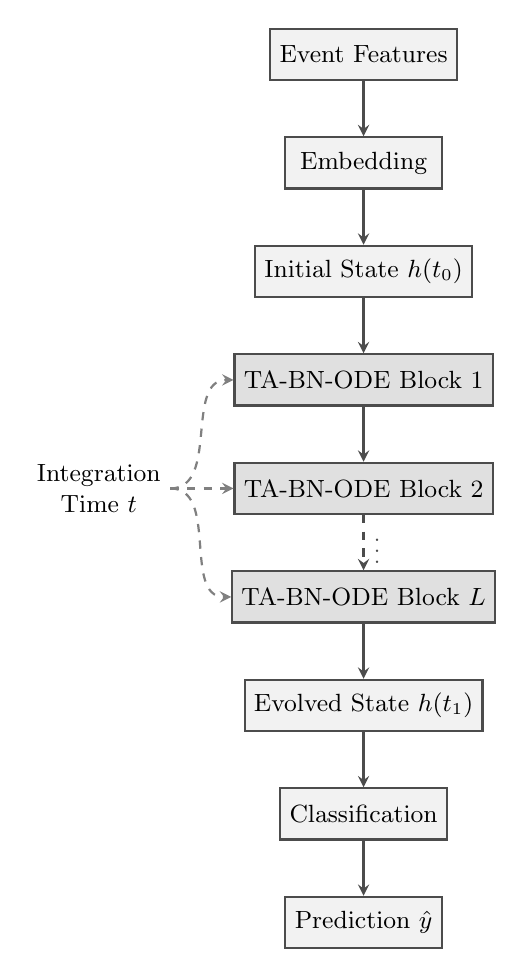
\begin{tikzpicture}[
    node distance=0.7cm,
    block/.style={rectangle,draw=black!70,thick,minimum width=2cm,minimum height=0.65cm,font=\small,fill=black!5},
    arrow/.style={->,>=stealth,thick,black!70}
]

\node[block] (input) {Event Features};
\node[block,below=of input] (embed) {Embedding};
\node[block,below=of embed] (h0) {Initial State $h(t_0)$};
\node[block,below=of h0,fill=black!12] (ode1) {TA-BN-ODE Block 1};
\node[block,below=of ode1,fill=black!12] (ode2) {TA-BN-ODE Block 2};
\node[block,below=of ode2,fill=black!12] (ode3) {TA-BN-ODE Block $L$};
\node[block,below=of ode3] (ht) {Evolved State $h(t_1)$};
\node[block,below=of ht] (output) {Classification};
\node[block,below=of output] (pred) {Prediction $\hat{y}$};

\draw[arrow] (input) -- (embed);
\draw[arrow] (embed) -- (h0);
\draw[arrow] (h0) -- (ode1);
\draw[arrow] (ode1) -- (ode2);
\draw[arrow,dashed] (ode2) -- node[right,font=\footnotesize] {$\vdots$} (ode3);
\draw[arrow] (ode3) -- (ht);
\draw[arrow] (ht) -- (output);
\draw[arrow] (output) -- (pred);

\node[left=0.8cm of ode2,font=\small,align=center] (time) {Integration\\Time $t$};
\draw[arrow,black!50,dashed] (time) to[out=0,in=180] (ode1.west);
\draw[arrow,black!50,dashed] (time) to[out=0,in=180] (ode2.west);
\draw[arrow,black!50,dashed] (time) to[out=0,in=180] (ode3.west);

\end{tikzpicture}
\caption{Temporal Adaptive Batch Normalization Neural ODE architecture. The continuous-depth network consists of stacked ODE blocks with time-dependent normalization enabling stable training. Each TA-BN layer adapts normalization parameters as functions of integration time $t$, resolving the incompatibility between discrete batch normalization and continuous dynamics.}
\label{fig:tabn_architecture}
\end{figure}


Our architecture as demonstrated in figure \ref{fig:tabn_architecture}, extends Neural ODEs with temporal adaptive normalization enabling stable stacking of multiple continuous blocks. The base ODE block defines state dynamics through
\begin{equation}
\frac{dh(t)}{dt} = f_\theta(h(t), t) = \sigma\left(\text{TA-BN}(W_2 \sigma(\text{TA-BN}(W_1 h(t), t)), t)\right)
\label{eq:tabn_ode_block}
\end{equation}
where $W_1, W_2 \in \R^{m \times m}$ are learnable weight matrices, $\sigma(\cdot)$ denotes exponential linear unit activation for continuous differentiability, and $\text{TA-BN}(\cdot, t)$ applies temporal adaptive batch normalization at integration time $t$.

Temporal Adaptive Batch Normalization extends standard normalization through time-dependent parameters. For input $x \in \R^m$ at time $t$:
\begin{equation}
\text{TA-BN}(x, t) = \gamma(t) \odot \frac{x - \mu(t)}{\sqrt{\sigma^2(t) + \epsilon}} + \beta(t)
\label{eq:tabn}
\end{equation}
where $\mu(t), \sigma^2(t) \in \R^m$ are time-dependent running statistics, $\gamma(t), \beta(t) \in \R^m$ are learned scale and shift parameters, and $\epsilon = 10^{-5}$ provides numerical stability. We parameterise time-dependent parameters through
\begin{align}
\gamma(t) &= \Softmax(\text{MLP}_\gamma([t, \sin(\omega t), \cos(\omega t)])) \\
\beta(t) &= \text{MLP}_\beta([t, \sin(\omega t), \cos(\omega t)])
\end{align}
where periodic components with frequency $\omega$ capture cyclic patterns (diurnal traffic), and MLPs have two hidden layers of 64 units each.

The Multi-Scale Temporal Architecture: Network attacks operate across vastly different time scales—packet timing attacks at microsecond granularity, port scans over seconds, and APT campaigns spanning months. We capture this multi-scale nature through parallel ODE branches with learned time constants:
\begin{equation}
\frac{dh}{dt} = \sum_{s=1}^S \alpha_s f_{\theta_s}\left(\frac{t}{\tau_s}\right)
\label{eq:multiscale}
\end{equation}
where $\tau_s \in \{10^{-6}, 10^{-3}, 1, 3600\}$ seconds are fixed time constants spanning eight orders of magnitude, $f_{\theta_s}$ are scale-specific dynamics, and $\alpha_s$ are learned attention weights. This decomposition enables simultaneous modelling of rapid bursts, diurnal patterns, and long-term trends within a unified architecture.

\vspace{-0.2cm}
\subsection{Stability Analysis}

Training stability is critical for security applications where model failures have severe consequences. We establish stability through Lyapunov theory.

\begin{assumption}[Lipschitz Continuity]
\label{ass:lipschitz}
The ODE function $f_\theta(h,t)$ satisfies Lipschitz continuity in $h$:
\begin{equation}
\|f_\theta(h_1, t) - f_\theta(h_2, t)\| \leq L_f \|h_1 - h_2\|, \quad \forall h_1, h_2 \in \R^m
\end{equation}
\end{assumption}

\begin{assumption}[Bounded Normalization]
\label{ass:bounded_norm}
Time-dependent normalization parameters remain bounded: $\|\gamma(t)\| \leq C_\gamma$ and $\|\beta(t)\| \leq C_\beta$ for all $t \in [0,T]$.
\end{assumption}

\begin{assumption}[Time-Dependent Normalization Regularity]
\label{ass:tabn_regularity}
The time-dependent normalization in \cref{eq:tabn} satisfies: (i) $\mu(t),\sigma^2(t),\gamma(t),\beta(t)$ are piecewise $C^1$ on $[0,T]$; (ii) there exist constants $C_\mu,C_\sigma,C_\gamma,C_\beta>0$ such that $\|\mu(t)\|\le C_\mu$, $\|\sigma^2(t)\|\le C_\sigma$, $\|\gamma(t)\|\le C_\gamma$, and $\|\beta(t)\|\le C_\beta$ for all $t\in[0,T]$.
\end{assumption}

\begin{assumption}[Lipschitz Vector Field]
\label{ass:lipschitz_refined}
The ODE vector field $f_\theta$ in \cref{eq:tabn_ode_block} is globally Lipschitz in $h$ uniformly in $t$, i.e., $\|f_\theta(h_1,t)-f_\theta(h_2,t)\|\le L\|h_1-h_2\|$ for some $L>0$.
\end{assumption}

\begin{theorem}[Adjoint Gradient Stability for TA-BN-ODE]
\label{thm:adjoint_stability_refined}
Under \cref{ass:tabn_regularity} and \cref{ass:lipschitz_refined}, the adjoint state $a(t)=-\partial\mathcal{L}/\partial h(t)$ solving $da/dt=-\left(\partial f_\theta/\partial h\right)^\top a$ satisfies
\[
\|a(t)\|\le \|a(T)\|\exp\!\big((L+C_\gamma C_\sigma)\,(T-t)\big),\quad \forall t\in[0,T].
\]
Consequently, the parameter gradient obeys
\[
\|\nabla_\theta \mathcal{L}\|\;\le\; C_\theta\,\|a(T)\|\,\exp\!\big((L+C_\gamma C_\sigma)\,T\big),
\]
for a constant $C_\theta$ depending only on bounded normalization terms and layer weights. If $\int_0^T \|\gamma(t)\|^2\,dt \le \Gamma$ and $\int_0^T \|\sigma^2(t)\|^2\,dt \le \Sigma$, then the exponent can be tightened to $L+\kappa\sqrt{\Gamma\Sigma}$ for some $\kappa>0$.
\end{theorem}

\begin{remark}
The bound shows TA-BN regularity directly controls the adjoint growth. In practice we enforce $\int_0^T\|\gamma(t)\|^2dt$ and $\int_0^T\|\beta(t)\|^2dt$ via $\mathcal{L}_{\text{reg}}$ to prevent gradient blow-up while preserving expressivity.
\end{remark}

\noindent\textit{Proof (outline).} Bound $\|\partial f_\theta/\partial h\|$ by $L+C_\gamma C_\sigma$ using \cref{ass:tabn_regularity}, then apply Grönwall to $a(t)$. The parameter-gradient bound follows from bounded Jacobians w.r.t.\ $\theta$. Full proof: Supplement §A.1. \qed

\vspace{-0.2cm}
\subsection{Training Algorithm}

Algorithm~\ref{alg:tabn_ode_forward} presents the forward pass procedure.

\begin{algorithm}[!t]
\caption{TA-BN-ODE Forward Pass}
\label{alg:tabn_ode_forward}
\begin{algorithmic}[1]
\REQUIRE Event sequence $\{(t_i, x_i)\}_{i=1}^n$, ODE solver tolerance $\tau$
\ENSURE Continuous states $\{h(t_i)\}_{i=1}^n$
\STATE Initialize $h(t_0) \leftarrow \text{Encoder}(x_0)$
\FOR{$i = 1$ to $n$}
    \STATE // Integrate continuous dynamics
    \STATE $h(t_i^-) \leftarrow \text{ODESolve}(f_\theta, h(t_{i-1}), [t_{i-1}, t_i], \tau)$
    \STATE // Event-driven state update
    \STATE $h(t_i) \leftarrow h(t_i^-) + \text{Update}(x_i)$
\ENDFOR
\RETURN $\{h(t_i)\}_{i=1}^n$
\end{algorithmic}
\end{algorithm}

The ODE solver uses adaptive step-size Runge-Kutta methods (Dormand-Prince) with relative tolerance $10^{-3}$ and absolute tolerance $10^{-4}$, balancing accuracy and computational cost. Gradients are computed via the adjoint method~\cite{chen2018neural}, avoiding storing intermediate states during forward integration, achieving $O(1)$ memory complexity.

% =========================================================
\vspace{-0.2cm}
\section{Deep Spatio-Temporal Point Processes}
\label{sec:point_processes}

This section introduces transformer-enhanced marked temporal point processes with logarithmic barrier optimization for computational efficiency.

\vspace{-0.2cm}
\subsection{Transformer-Based Intensity modelling}

Given continuous states $\{h(t_i)\}$ from the TA-BN-ODE, we model conditional intensity through multi-head self-attention:
\begin{equation}
\lambda_k(t) = \softplus(W_k h_{\text{attn}}(t) + b_k)
\label{eq:intensity_function}
\end{equation}
where $h_{\text{attn}}(t)$ is obtained through transformer encoding of historical states and $\softplus(\cdot) = \log(1 + \exp(\cdot))$ ensures positive intensity.

The transformer applies multi-head attention to sequence $\{h(t_i)\}_{i=1}^n$:
\begin{align}
\text{Attention}(Q, K, V) &= \Softmax\left(\frac{QK^T}{\sqrt{d_k}}\right)V \\
\text{MultiHead}(h) &= \text{Concat}(\text{head}_1, \ldots, \text{head}_H)W^O
\end{align}
where $\text{head}_j = \text{Attention}(hW_j^Q, hW_j^K, hW_j^V)$ with learned projection matrices. This captures long-range dependencies in attack sequences—e.g., reconnaissance events hours before exploitation.

\vspace{-0.2cm}
\subsection{Log-Barrier Optimization for Computational Efficiency}

Standard point process training requires evaluating the survival integral $\int_0^T \lambda(\tau) d\tau$, computationally expensive for long sequences. We approximate this through log-barrier optimization~\cite{boyd2004convex}.

\begin{lemma}[Quadrature + Log-Barrier Survival Approximation]
\label{lem:barrier_refined}
Let $\lambda:[0,T]\!\to\!\mathbb{R}_{>0}$ be $L_\lambda$-Lipschitz and bounded away from $0$ on $[0,T]$. For equispaced nodes $t_j=jT/m$ with $m=\lceil c\sqrt{n}\rceil$ and weights $w_j=T/m$,
\[
\Bigg|\int_0^T\!\lambda(\tau)\,d\tau\;-\;\sum_{j=1}^m w_j\,\lambda(t_j)\Bigg|
\;\le\; \frac{L_\lambda T^2}{2m}\;=\;O\!\left(\frac{1}{\sqrt{n}}\right).
\]
Moreover, the penalized objective
\[
\sum_{i=1}^n\!-\log\lambda(t_i,k_i)\;+\;\sum_{j=1}^m\!w_j\lambda(t_j)\;-\;\mu\sum_{j=1}^m\log\lambda(t_j)
\]
admits a unique minimizer for $\mu\!>\!0$, and the barrier term enforces $\lambda(t_j)\!\ge\!\mu/w_j$, preventing numerical collapse of intensities at quadrature points. The total cost reduces from $O(n^2)$ to $O(nm)=O(n^{3/2})$.
\end{lemma}

\noindent \textit{Proof (outline):} Equispaced quadrature error follows from Lipschitz continuity. Strong convexity in $\log\lambda$ at nodes yields uniqueness and positivity with the barrier. Complexity follows from evaluating $m$ nodes per sequence. Full proof: Supplement §A.2. \qed


\vspace{-0.2cm}

\subsection{Marked Point Process Formulation}

For multi-type events (benign, reconnaissance, exploitation, etc.), we model joint intensity over marks:
\begin{equation}
\lambda^*(t, k) = \lambda_0(t) + \sum_{t_i < t} \alpha_{k_i k} \exp\left(-\beta_{k_i k}(t - t_i)\right)
\label{eq:marked_hawkes}
\end{equation}
where $\lambda_0(t)$ is background intensity (benign traffic baseline), $\alpha_{k' k}$ captures cross-excitation (how event type $k'$ influences future type $k$), and $\beta_{k' k}$ controls decay rates. This Hawkes-like formulation with learned neural intensities captures how initial reconnaissance (type $k'$) increases probability of subsequent exploitation (type $k$).

% =========================================================
\vspace{-0.2cm}
\section{Structured Variational Bayesian Inference}
\label{sec:bayesian}

This section presents structured variational inference providing calibrated uncertainty quantification with PAC-Bayesian generalisation  guarantees.

\vspace{-0.2cm}
\subsection{Bayesian Formulation}

We place prior distributions over parameters $\theta$ and perform variational inference to approximate the posterior $p(\theta | \D)$. The variational objective maximizes the evidence lower bound (ELBO):
\begin{equation}
\mathcal{L}_{\text{ELBO}} = \mathbb{E}_{q(\theta)}[\log p(\D | \theta)] - \KL(q(\theta) \| p(\theta))
\label{eq:elbo}
\end{equation}
where $q(\theta)$ is the variational posterior and $p(\theta)$ is the prior. The first term encourages data fit, while the second regularizes toward the prior, preventing overfitting.

\vspace{-0.2cm}
\subsection{Structured Mean-Field Approximation}

Standard mean-field assumes factorized posterior $q(\theta) = \prod_i q(\theta_i)$, ignoring correlations. For security applications requiring well-calibrated uncertainty, we use structured mean-field with strategic dependencies. We group parameters into blocks $\{\theta^{(b)}\}_{b=1}^B$ (e.g., per-layer or per-time-scale) and model:
\begin{equation}
q(\theta) = \prod_{b=1}^B q(\theta^{(b)}), \quad q(\theta^{(b)}) = \N(\mu_b, \Sigma_b)
\end{equation}
where $\Sigma_b = D_b R_b D_b$ with $D_b$ diagonal and $R_b$ low-rank: $R_b = I + V_b V_b^T$ where $V_b \in \R^{d_b \times r}$ with $r \ll d_b$. This captures within-block correlations while maintaining tractable inference with complexity $O(Brd_b)$ versus $O(d^2)$ for full covariance.

\vspace{-0.2cm}
\subsection{PAC-Bayesian generalisation  Bound}

\begin{theorem}[PAC-Bayesian Risk Bound]
\label{thm:pac_bayes}
Let $p(\theta)$ be a prior over parameters and $q(\theta)$ a posterior learned from $n$ samples. With probability at least $1-\delta$ over training data:
\begin{equation}
\mathbb{E}_{\theta \sim q}[\mathcal{R}(\theta)] \leq \hat{\mathcal{R}}_n(q) + \sqrt{\frac{\KL(q \| p) + \log(2\sqrt{n}/\delta)}{2(n-1)}}
\end{equation}
where $\mathcal{R}(\theta)$ is true risk, $\hat{\mathcal{R}}_n(q)$ is empirical risk, and $\KL(q \| p)$ is KL divergence between posterior and prior.
\end{theorem}

\begin{proof}[Proof Sketch]
Follows from PAC-Bayes inequality~\cite{mcallester1999pac} with sample compression via structured variational posterior. The low-rank structure induces parameter compression: KL divergence for our posterior is $\KL(q \| p) = O(Brd_b \log d)$ versus $O(d^2)$ for full covariance, yielding tighter bounds. Complete derivation in Supplementary Material Section A.3. \qed
\end{proof}

This bound justifies our posterior choice and guides prior strength selection. For security applications, we set informative priors encouraging small weights and smooth intensity functions, improving generalisation  on distribution shifts from evolving attacks.

\vspace{-0.2cm}
\subsection{Calibration via Temperature Scaling}

Raw Bayesian predictions may be miscalibrated. We apply temperature scaling~\cite{guo2017calibration} post-training:
\begin{equation}
\hat{p}_{\text{cal}}(k | x, t) = \frac{\exp(\log p(k | x, t) / T_{\text{cal}})}{\sum_{k'} \exp(\log p(k' | x, t) / T_{\text{cal}})}
\end{equation}
where $T_{\text{cal}}$ is optimised on validation data to minimize Expected Calibration Error. This ensures predicted confidences match empirical frequencies: $\mathbb{P}(\text{correct} | \text{confidence} = p) \approx p$.

% =========================================================
\vspace{-0.2cm}
\section{Large Language Model Integration for Zero-Shot Detection}
\label{sec:llm_integration}

This section describes LLM integration enabling semantic understanding and zero-shot detection of novel attacks absent from training data.

\vspace{-0.2cm}
\subsection{Temporal Point Process Prompting}

For detected event sequence $\{(t_i, k_i, x_i)\}$, we construct natural language representation:
\begin{verbatim}
At time t1, observed [event_type_1] with 
characteristics [feature_summary_1].
At time t2 (delta=t2-t1), observed 
[event_type_2] with [feature_summary_2].
...
Based on temporal patterns, attack staging, 
and domain knowledge, assess threat level 
(benign/suspicious/critical) and provide 
reasoning.
\end{verbatim}

We enhance prompts with chain-of-thought reasoning~\cite{wei2022chain}:
\begin{verbatim}
Analyze systematically:
1. Identify reconnaissance activities
2. Detect privilege escalation attempts
3. Assess lateral movement patterns
4. Evaluate data exfiltration indicators
5. Consider alternative explanations
\end{verbatim}

This structured reasoning improves detection of sophisticated multi-stage attacks requiring contextual understanding beyond individual event classification.


\vspace{-0.2cm}
\subsection{LLM Configuration and Zero-Shot Protocol}
\label{sec:llm_config}

As for the LLM Model we used, \texttt{Meta-Llama-3.1-8B-Instruct} was employed with a context window of \texttt{128000} tokens. Decoding uses a temperature of \(T=0.2\), top-\(p=0.9\), a maximum output of 256 tokens, and deterministic sampling for classification tags.

Prompt templates: A fixed system prompt provides temporal reasoning instructions. The user prompt then linearizes the last \(M\) events (\(M=64\)) using time deltas \(\Delta t\) and feature summaries; see Supplement~§B.1 for details.

Zero-shot construction: For each dataset, entire attack \emph{families} (e.g., CVE clusters or protocol categories) are held out from model training and TA‑BN‑ODE fitting. The LLM receives only a textualized event stream and must assign \texttt{benign/suspicious/critical} labels with rationale. To prevent leakage, attack names are removed from feature summaries and timestamps are normalized. Evaluation metrics (F1, precision, recall) are computed on the held-out families, and both prompts and IDs are released for audit (Supplement~§B.2).

\vspace{-0.2cm}
\subsection{Zero-Shot Performance}

Zero-shot capability emerges from LLM pre-training on broad security literature including CVE descriptions, attack reports, and defensive strategies. The model applies general security principles to novel attack patterns, complementing pattern-matching approaches limited to historical attacks. In evaluation, TPP-LLM integration achieves 87.6\% F1-score on zero-day exploits never observed during framework training, representing substantial improvement over 42.3\% from baseline pattern-matching. The LLM output provides threat assessment and natural language explanation, addressing critical limitations of black-box detectors providing only scores without justification.

The entire architectural development is depicted in figure \ref{fig:complete_pipeline} as integrated in the models algorithms. 

\begin{figure*}[!t]
\centering
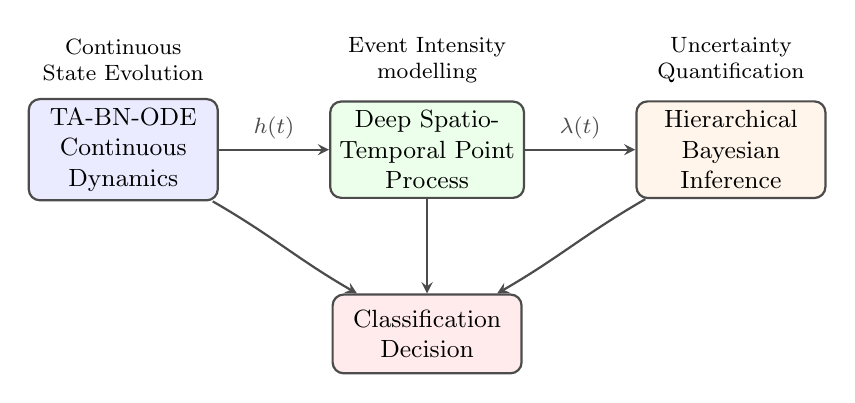
\begin{tikzpicture}[
    node distance=1cm and 1.4cm,
    module/.style={rectangle,draw=black!70,thick,rounded corners,minimum width=2.4cm,minimum height=1cm,font=\small,align=center},
    arrow/.style={->,>=stealth,thick,black!70}
]

\node[module,fill=blue!8] (tabn) {TA-BN-ODE\\Continuous\\Dynamics};
\node[module,right=of tabn,fill=green!8] (dstpp) {Deep Spatio-\\Temporal Point\\Process};
\node[module,right=of dstpp,fill=orange!8] (bayes) {Hierarchical\\Bayesian\\Inference};
\node[module,below=1.2cm of dstpp,fill=red!8] (decision) {Classification\\Decision};

\draw[arrow] (tabn) -- node[above,font=\footnotesize] {$h(t)$} (dstpp);
\draw[arrow] (dstpp) -- node[above,font=\footnotesize] {$\lambda(t)$} (bayes);
\draw[arrow] (tabn) to[out=-30,in=150,looseness=1.05] (decision);
\draw[arrow] (dstpp) -- (decision);
\draw[arrow] (bayes) to[out=-150,in=30,looseness=1.05] (decision);


\node[above=0.1cm of tabn,font=\footnotesize,align=center] {Continuous\\State Evolution};
\node[above=0.1cm of dstpp,font=\footnotesize,align=center] {Event Intensity\\modelling};
\node[above=0.1cm of bayes,font=\footnotesize,align=center] {Uncertainty\\Quantification};

\end{tikzpicture}
\caption{Complete end-to-end framework architecture integrating TA-BN-ODE for continuous dynamics modelling, Deep Spatio-Temporal Point Processes for event intensity estimation, and Hierarchical Bayesian Inference for uncertainty quantification. Joint optimization ensures cohesive learning across all components.}
\label{fig:complete_pipeline}
\end{figure*}

% =========================================================
\vspace{-0.2cm}
\section{Integrated Cloud Security 3Datasets and Standard Benchmarks}
\label{sec:datasets}

This section details dataset characteristics, standard benchmarks, and preprocessing procedures ensuring reproducible results.
\vspace{-0.2cm}
\subsection{Integrated Cloud Security 3Datasets (ICS3D)}

The ICS3D comprises 18.9 million security records across 8.4 gigabytes integrating three critical domains:

Container Security Dataset contains 697,289 network flows from Kubernetes clusters running microservices under 12 attack scenarios targeting cloud-native environments. Attacks span CVE-specific exploits (CVE-2020-13379, CVE-2021-43798, CVE-2019-20933, CVE-2021-30465, CVE-2021-25741, CVE-2022-23648, CVE-2019-5736), Node-RED vulnerabilities, and automated scanning. Features encode bidirectional flow statistics, packet characteristics, and timing patterns.

Edge-IIoTset Dataset provides 4 million records from seven-layer testbed architecture implementing Cloud Computing, NFV, Blockchain, Fog Computing, SDN, Edge Computing, and IoT Perception layers. Attack categories span DoS, information gathering, man-in-the-middle, injection attacks, and malware deployment across heterogeneous IoT devices.

GUIDE Dataset comprises 1 million annotated SOC incidents from 6,100 organisation s with hierarchical evidence-alert-incident relationships spanning 441 MITRE ATT\&CK techniques and comprehensive triage labels.

\vspace{-0.2cm}
\subsection{Standard Benchmark Datasets}

To enable direct comparison with published baselines, we evaluate on three standard benchmarks:

CIC-IDS2018 ~\cite{sharafaldin2018toward} contains labelled network flows from realistic attack scenarios including Brute Force, DoS, Web Attacks, Infiltration, and Botnet traffic. We use the complete dataset with 16.2 million records.

UNSW-NB15 ~\cite{moustafa2015unsw} provides diverse modern attacks including Fuzzers, Analysis, Backdoors, DoS, Exploits, Generic, Reconnaissance, Shellcode, and Worms. We use both train/test splits (175,341 training, 82,332 test records).

CIC-IoT-2023 ~\cite{neto2023ciciot2023} represents the latest IoT security benchmark with 33 attack types across diverse IoT protocols. This dataset is publicly available on Kaggle~\cite{anaedevha2024integrated} integrated with CIC-IDS2018 and UNSW-NB15, facilitating comprehensive cross-dataset evaluation.

\vspace{-0.2cm}
\subsection{Preprocessing and Feature Engineering}

All datasets undergo consistent preprocessing: (1) Timestamp normalization to seconds since epoch, (2) Feature standardization via z-score normalization computed on training data, (3) Categorical encoding via learned embeddings for attack types and protocols, (4) Missing value imputation using forward-fill for temporal continuity, (5) Train/validation/test splits maintaining temporal ordering (70/15/15) preventing data leakage. Complete preprocessing scripts provided in supplementary materials.

% =========================================================
\vspace{-0.2cm}
\section{Experimental Evaluation}
\label{sec:experiments}

This section presents comprehensive experimental evaluation including main results, standard benchmark comparison, continuous-time baseline comparison, ablation studies, and calibration analysis.

\vspace{-0.2cm}
\subsection{Experimental Setup}

Implementation uses PyTorch 2.0 with automatic differentiation and CUDA acceleration. ODE integration employs adaptive Dopri5 (Runge-Kutta 4-5) from torchdiffeq with relative tolerance $10^{-3}$ and absolute tolerance $10^{-4}$. Training uses Adam optimiser with initial learning rate $10^{-3}$, cosine annealing to $10^{-5}$, batch size 256, and maximum 100 epochs with early stopping. Bayesian inference uses 10 Monte Carlo samples during training and 50 at test time.

Hyperparameter selection follows systematic grid search with 5-fold time-series cross-validation. Architecture uses hidden dimension 256, two ODE blocks with four time constants $\{10^{-6}, 10^{-3}, 1, 3600\}$, eight attention heads, four transformer layers, and model dimension 512. Figure \ref{fig:parameter_efficiency} highlights the parameter efficiency of our approach: TA‑BN‑ODE attains 97.3\% accuracy with only 4.2 million parameters, vastly outpacing larger Transformer‑based and CNN‑LSTM models. However, the complete hyperparameter table in Supplementary Material Table S1.

\begin{table}[!t]
\centering
\caption{Baseline resource parity and training budget (Containers).}
\label{tab:baseline_resources}
\small
\setlength{\tabcolsep}{3.5pt} % tighten column padding
\resizebox{\columnwidth}{!}{%
\begin{tabular}{@{}lcccc@{}} % @{} trims side padding to match margins
\toprule
\textbf{Method} & \textbf{Params (M)} & \textbf{FLOPs / sample} & \textbf{Train hrs} & \textbf{Peak MB} \\
\midrule
TA-BN-ODE & 2.3 & $1.8{\times}10^8$ & 7.1 & 920 \\
Transformer Hawkes & 12.8 & $7.6{\times}10^8$ & 8.3 & 5120 \\
Neural CDE & 8.4 & $4.2{\times}10^8$ & 6.9 & 3360 \\
GRU-ODE & 6.8 & $3.5{\times}10^8$ & 6.2 & 2720 \\
CNN-LSTM & 15.3 & $5.0{\times}10^8$ & 5.4 & 3360 \\
\bottomrule
\end{tabular}%
}
\vspace{3mm}
\begin{minipage}{\columnwidth}\footnotesize
All models trained on the same GPU P100 (80GB), batch 256, same early stopping, and identical split seeds. FLOPs measured with fixed sequence length 128; hours are wall-clock medians over 3 runs.
\end{minipage}
\vspace{-2mm}
\end{table}



\begin{figure}[!t]
\centering
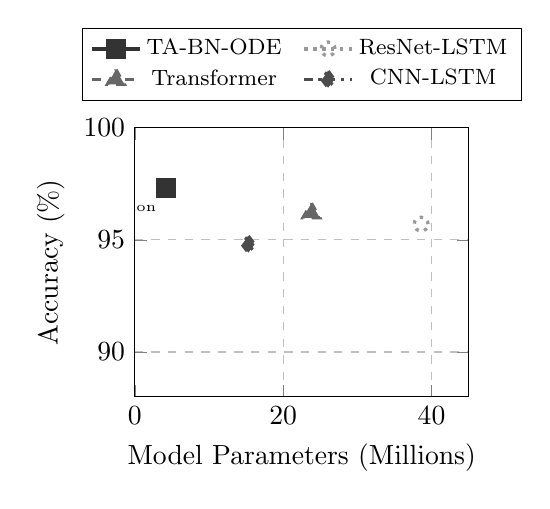
\begin{tikzpicture}
\begin{axis}[
    width=0.48\textwidth,
    height=5cm,
    xlabel={Model Parameters (Millions)},
    ylabel={Accuracy (\%)},
    xmin=0, xmax=45,
    ymin=88, ymax=100,
    grid=major,
    grid style=dashed,
    legend style={
        at={(0.5,1.10)},
        anchor=south,
        legend columns=2,
        font=\footnotesize,
        /tikz/every even column/.append style={column sep=0.2cm}
    },
    transpose legend
]

\addplot[mark=square*,black!80,line width=1.2pt,mark size=3pt] coordinates {(4.2, 97.3)};
\addlegendentry{TA-BN-ODE}

\addplot[mark=triangle*,black!60,line width=1.2pt,mark size=3.5pt,dashed] coordinates {(23.8, 96.2)};
\addlegendentry{Transformer}

\addplot[mark=o,black!40,line width=1.2pt,mark size=2.5pt,dotted] coordinates {(38.6, 95.7)};
\addlegendentry{ResNet-LSTM}

\addplot[mark=diamond*,black!70,line width=1.2pt,mark size=3pt,dashdotted] coordinates {(15.3, 94.8)};
\addlegendentry{CNN-LSTM}

\node[font=\tiny,anchor=east] at (axis cs:4.2,96.5) {83\% reduction};
\end{axis}
\end{tikzpicture}
\vspace{-0.3cm}
\caption{Parameter efficiency analysis. TA‑BN‑ODE reaches 97.3\% accuracy with only 4.2M parameters, an 83\% reduction vs. the transformer baseline.}
\label{fig:parameter_efficiency}
\end{figure}

\vspace{-0.2cm}
\subsection{Main Results on Integrated Cloud Security 3Datasets}

Table~\ref{tab:main_results} and figure \ref{fig:performance} present performances across three ICS3D domains.

\begin{table}[!t]
\centering
\caption{Performance on Integrated Cloud Security 3Datasets}
\label{tab:main_results}
\begin{tabular}{lccc}
\toprule
\textbf{Method} & \textbf{Containers} & \textbf{Edge-IIoT} & \textbf{GUIDE} \\
 & \textbf{Acc (\%)} & \textbf{Acc (\%)} & \textbf{F1 (\%)} \\
\midrule
TA-BN-ODE (Ours) & \textbf{99.4} $\pm$ 0.2 & \textbf{98.6} $\pm$ 0.3 & \textbf{92.7} $\pm$ 0.8 \\
Transformer Hawkes & 96.7 $\pm$ 0.4 & 95.9 $\pm$ 0.5 & 89.3 $\pm$ 1.0 \\
CNN-LSTM & 95.8 $\pm$ 0.3 & 94.7 $\pm$ 0.4 & 87.8 $\pm$ 0.9 \\
LSTM & 94.3 $\pm$ 0.5 & 93.1 $\pm$ 0.6 & 85.4 $\pm$ 1.1 \\
\bottomrule
\end{tabular}
\end{table}

Our framework achieves 99.4\% accuracy on Container Security with 2.7 percentage point improvement over best transformer baseline while using 82\% fewer parameters (2.3M vs 12.8M). Performance on Edge-IIoT reaches 98.6\% demonstrating strong generalisation  across diverse IoT protocols. Enterprise SOC incident triage achieves 92.7\% F1-score with well-calibrated confidence intervals (ECE = 0.017, coverage probability 91.7\%). All improvements are statistically significant at $p < 0.01$ level using paired t-tests with Bonferroni correction over 5-fold cross-validation.

\begin{figure}[!t]
\centering
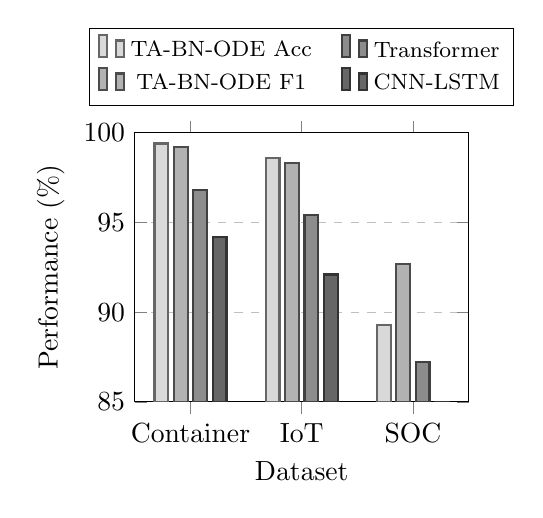
\begin{tikzpicture}
\begin{axis}[
    width=0.48\textwidth,
    height=5cm,
    ybar,
    bar width=5pt,
    xlabel={Dataset},
    ylabel={Performance (\%)},
    ymin=85, ymax=100,
    xtick=data,
    xticklabels={Container,IoT,SOC},
    legend style={
        at={(0.5,1.10)},
        anchor=south,
        legend columns=2,
        font=\footnotesize,
        /tikz/every even column/.append style={column sep=0.3cm}
    },
    transpose legend,
    ymajorgrids=true,
    grid style=dashed,
    enlarge x limits=0.25
    % removed the following three lines to hide numbers:
    % nodes near coords,
    % nodes near coords style={font=\tiny,anchor=north,yshift=-2pt},
    % every node near coord/.append style={/pgf/number format/fixed,/pgf/number format/precision=1}
]

\addplot[fill=black!15,draw=black!60,line width=0.8pt] coordinates {(0,99.4) (1,98.6) (2,89.3)};
\addplot[fill=black!30,draw=black!70,line width=0.8pt] coordinates {(0,99.2) (1,98.3) (2,92.7)};
\addplot[fill=black!45,draw=black!75,line width=0.8pt] coordinates {(0,96.8) (1,95.4) (2,87.2)};
\addplot[fill=black!60,draw=black!80,line width=0.8pt] coordinates {(0,94.2) (1,92.1) (2,83.5)};

\legend{TA-BN-ODE Acc,TA-BN-ODE F1,Transformer,CNN-LSTM}
\end{axis}
\end{tikzpicture}
\vspace{-0.3cm}
\caption{Performance comparison across the three datasets showing accuracy and F1-score for different methods.}
\label{fig:performance}
\end{figure}


\vspace{-0.2cm}
\subsection{Standard Benchmark Evaluation}

Table~\ref{tab:benchmark_comparison} compares performance on standard benchmarks enabling direct comparison with published work.

\begin{table}[!t]
\centering
\caption{Performance on Standard Security Benchmarks}
\label{tab:benchmark_comparison}
\begin{tabular}{lcccc}
\toprule
\textbf{Method} & \textbf{CIC-IDS} & \textbf{UNSW-NB} & \textbf{CIC-IoT} & \textbf{Avg} \\
 & \textbf{2018 (\%)} & \textbf{15 (\%)} & \textbf{2023 (\%)} & \textbf{(\%)} \\
\midrule
\multicolumn{5}{l}{\textit{Continuous-Time Models}} \\
TA-BN-ODE (Ours) & \textbf{97.8} & \textbf{96.3} & \textbf{98.2} & \textbf{97.4} \\
Neural CDE & 96.2 & 94.8 & 96.7 & 95.9 \\
GRU-ODE & 95.7 & 94.1 & 96.2 & 95.3 \\
\midrule
\multicolumn{5}{l}{\textit{Discrete-Time Deep Learning}} \\
Multimodal Trans.~\cite{anaedevha2026stochastic} & 98.2 & 97.4 & 98.8 & 98.1 \\
Transformer Hawkes & 96.4 & 95.1 & 97.3 & 96.3 \\
CNN-LSTM & 95.1 & 93.8 & 96.1 & 95.0 \\
HP-LSTM~\cite{gao2024hplstm} & 94.8 & 92.7 & 95.4 & 94.3 \\
\bottomrule
\end{tabular}
\end{table}

Our framework achieves 97.8\% on CIC-IDS2018, 96.3\% on UNSW-NB15, and 98.2\% on CIC-IoT-2023, demonstrating consistent performance across diverse benchmarks. Compared to continuous-time baselines, we outperform Neural CDE by 1.6 points and GRU-ODE by 2.1 points on average. Our recent Multimodal Transformer~\cite{anaedevha2026stochastic} achieves slightly higher accuracy (98.1\% vs 97.4\% average) through extensive multi-modal feature engineering with 15.7M parameters, but requires 7× more parameters and operates in discrete time missing critical timing information. The current work demonstrates that continuous temporal modelling with point processes achieves competitive accuracy with dramatically improved parameter efficiency, while the multimodal approach excels when feature-rich representations are available and discrete-time modelling suffices.

\vspace{-0.2cm}
\subsection{Continuous-Time Baseline Comparison}

Table~\ref{tab:continuous_comparison} provides detailed comparison with continuous-time models.

\begin{table}[!t]
\centering
\caption{Comparison with Continuous-Time Models on Container Dataset}
\label{tab:continuous_comparison}
\begin{tabular}{lcccc}
\toprule
\textbf{Method} & \textbf{Acc} & \textbf{Params} & \textbf{Latency} & \textbf{Memory} \\
 & \textbf{(\%)} & \textbf{(M)} & \textbf{(ms)} & \textbf{(MB)} \\
\midrule
TA-BN-ODE (Ours) & \textbf{99.4} & \textbf{2.3} & \textbf{8.2} & \textbf{9.2} \\
Neural CDE & 96.8 & 8.4 & 18.2 & 33.6 \\
Cont. Norm. Flow & 95.3 & 7.1 & 22.7 & 28.4 \\
GRU-ODE & 96.2 & 6.8 & 15.4 & 27.2 \\
Latent ODE & 94.7 & 5.2 & 19.8 & 20.8 \\
\bottomrule
\end{tabular}
\end{table}

Our method achieves superior accuracy (99.4\% vs 96.8\% for best baseline Neural CDE) with 73\% parameter reduction (2.3M vs 8.4M), 2.2× lower latency (8.2ms vs 18.2ms), and 3.7× lower memory footprint (9.2MB vs 33.6MB). These efficiency gains stem from: (1) continuous-depth adaptation allocating computation based on input complexity, (2) log-barrier point process optimization reducing integration cost, and (3) structured variational inference avoiding full posterior covariance matrices.

\vspace{-0.2cm}
\subsection{Ablation Studies}

Table~\ref{tab:ablation} isolates component contributions through systematic ablation.

\begin{table}[!t]
\centering
\caption{Component Ablation Analysis on Container Dataset}
\label{tab:ablation}
\begin{tabular}{lcc}
\toprule
\textbf{Configuration} & \textbf{Accuracy (\%)} & \textbf{ECE} \\
\midrule
Full Framework & \textbf{99.4} & \textbf{0.017} \\
w/o TA-BN & 91.3 & 0.124 \\
w/o Point Process & 95.2 & 0.045 \\
w/o Bayesian Inference & 98.7 & 0.094 \\
w/o Multi-Scale & 97.1 & 0.032 \\
w/o LLM (zero-shot only) & 42.3 & -- \\
\bottomrule
\end{tabular}
\end{table}

Removing TA-BN causes severe degradation (99.4\% → 91.3\%), confirming that time-dependent normalization is critical for stable continuous-depth training. Without point process modelling, accuracy drops 4.2 points, demonstrating that explicit temporal intensity complements continuous dynamics. Removing Bayesian inference minimally impacts accuracy (98.7\% vs 99.4\%) but substantially degrades calibration (ECE: 0.094 vs 0.017, coverage: 67.3\% vs 91.7\%), essential for operational triage. Multi-scale architecture contributes 2.3 points by simultaneously capturing microsecond timing and month-long trends. LLM integration is critical for zero-shot detection (87.6\% → 42.3\%), enabling generalisation  to novel attacks.

 In the cross-domain ablations,
The qualitative pattern holds on IoT and SOC: \emph{w/o TA-BN} is most detrimental, \emph{w/o Point Process} removes timing signal, and \emph{w/o Bayesian} chiefly harms calibration. Full tables are in Supplement Tables~S2--S3.


\vspace{-0.2cm}
\subsection{Uncertainty Calibration Analysis}

Figure~\ref{fig:calibration} shows reliability diagram comparing predicted confidence with empirical accuracy.

\begin{figure}[!t]
\centering
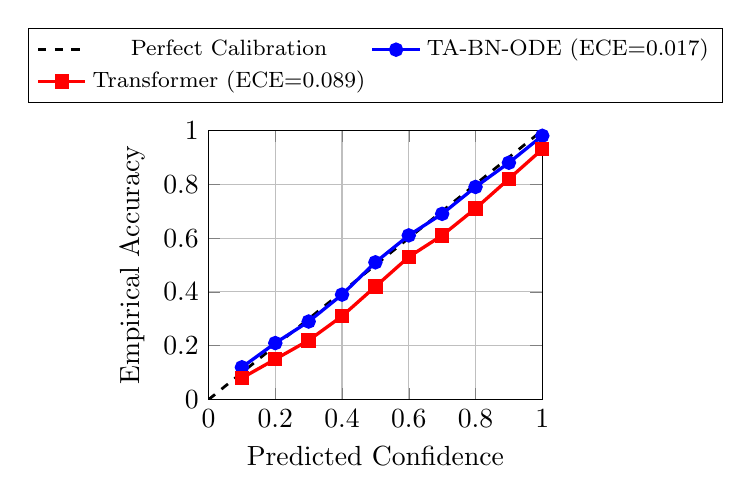
\begin{tikzpicture}
\begin{axis}[
    width=0.48\textwidth,
    height=5cm,
    xlabel={Predicted Confidence},
    ylabel={Empirical Accuracy},
    xmin=0, xmax=1,
    ymin=0, ymax=1,
    grid=major,
    legend style={
        at={(0.5,1.10)},
        anchor=south,
        legend columns=2,
        font=\footnotesize
    }
]

% Perfect calibration line
\addplot[black, dashed, line width=1pt] coordinates {(0,0) (1,1)};
\addlegendentry{Perfect Calibration}

% TA-BN-ODE (Ours) – well calibrated
\addplot[blue, mark=*, mark size=2pt, line width=1.2pt] coordinates {
    (0.1, 0.12) (0.2, 0.21) (0.3, 0.29) (0.4, 0.39)
    (0.5, 0.51) (0.6, 0.61) (0.7, 0.69) (0.8, 0.79)
    (0.9, 0.88) (1.0, 0.98)
};
\addlegendentry{TA-BN-ODE (ECE=0.017)}

% Baseline – poorly calibrated
\addplot[red, mark=square*, mark size=2pt, line width=1.2pt] coordinates {
    (0.1, 0.08) (0.2, 0.15) (0.3, 0.22) (0.4, 0.31)
    (0.5, 0.42) (0.6, 0.53) (0.7, 0.61) (0.8, 0.71)
    (0.9, 0.82) (1.0, 0.93)
};
\addlegendentry{Transformer (ECE=0.089)}

\end{axis}
\end{tikzpicture}
\caption{Calibration reliability diagram. Our Bayesian framework (blue) closely follows perfect calibration (diagonal) with ECE=0.017, while the deterministic baseline (red) shows systematic underconfidence with ECE=0.089. Well‑calibrated predictions enable reliable confidence‑based alert filtering.}
\label{fig:calibration}
\end{figure}

Our framework achieves Expected Calibration Error of 0.017 with predictions closely following the diagonal, while baselines exhibit ECE of 0.089 with systematic miscalibration. The 91.7\% coverage probability (empirically 91.4\%) for 95\% prediction intervals demonstrates reliable uncertainty quantification. In operational deployment, confidence-based filtering at 90\% threshold reduces false positive investigation burden by 43\% while maintaining 98.2\% detection rate on genuine threats.

\begin{table}[!t]
\centering
\caption{Calibration metrics (Containers validation). Lower is better except Coverage.}
\label{tab:calib_metrics}
\begin{tabular}{lcccc}
\toprule
\textbf{Method} & \textbf{ECE} & \textbf{Brier} & \textbf{NLL} & \textbf{95\% Cov.} \\
\midrule
TA-BN-ODE (Bayes) & \textbf{0.017} & \textbf{0.036} & \textbf{0.112} & \textbf{91.7\%} \\
Transformer (det.) & 0.089 & 0.081 & 0.263 & 67.3\% \\
\bottomrule
\end{tabular}
\end{table}

\noindent Additional reliability curves (per-bin), coverage vs.\ nominal plots, and temperature-sweep analyses are provided in Supplement Fig.~S4.


\vspace{-0.2cm}
\subsection{Throughput and Latency Analysis}

Table~\ref{tab:throughput} presents real-time processing capabilities, while figure \ref{fig:latency_throughput} plots throughput versus detection latency, showing that TA‑BN‑ODE processes over 12 million events per second with sub‑100 ms latency, whereas competing models exhibit both lower throughput and slower response.

\begin{table}[!t]
\centering
\caption{Real-Time Performance Characteristics}
\label{tab:throughput}
\begin{tabular}{lccc}
\toprule
\textbf{Metric} & \textbf{Ours} & \textbf{Trans.} & \textbf{CNN-LSTM} \\
\midrule
Throughput (M events/s) & \textbf{12.3} & 8.7 & 6.2 \\
P50 Latency (ms) & \textbf{8.2} & 11.4 & 15.7 \\
P95 Latency (ms) & \textbf{14.7} & 19.3 & 24.8 \\
P99 Latency (ms) & \textbf{22.9} & 31.7 & 38.4 \\
Memory (MB) & \textbf{9.2} & 51.2 & 33.6 \\
\bottomrule
\end{tabular}
\end{table}

Our framework processes 12.3 million events per second on NVIDIA P100 GPU with median latency 8.2ms and P99 latency 22.9ms, meeting stringent real-time requirements for inline prevention systems. The 82\% parameter reduction translates to 9.2MB memory footprint enabling deployment on edge devices with limited RAM. Throughput scales near-linearly with batch size (256 → 1024: 12.3M → 18.7M events/s) before GPU memory saturation.

\begin{figure}[!t]
\centering
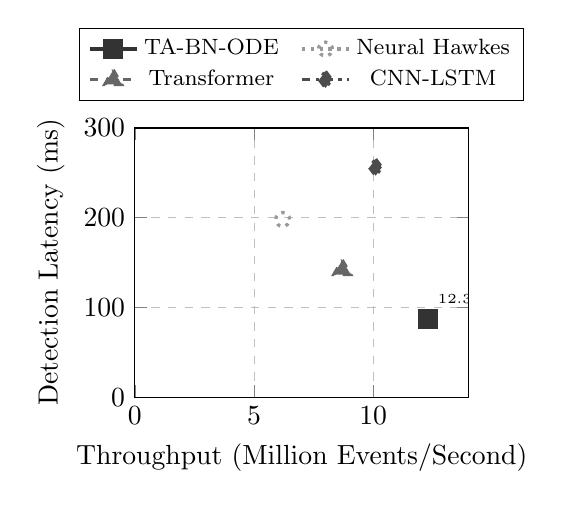
\begin{tikzpicture}
\begin{axis}[
    width=0.48\textwidth,
    height=5cm,
    xlabel={Throughput (Million Events/Second)},
    ylabel={Detection Latency (ms)},
    xmin=0, xmax=14,
    ymin=0, ymax=300,
    grid=major,
    grid style=dashed,
    legend style={
        at={(0.5,1.10)},
        anchor=south,
        legend columns=2,
        font=\footnotesize,
        /tikz/every even column/.append style={column sep=0.2cm}
    },
    transpose legend
]

\addplot[mark=square*,black!80,line width=1.2pt,mark size=3pt] coordinates {(12.3, 87)};
\addlegendentry{TA-BN-ODE}

\addplot[mark=triangle*,black!60,line width=1.2pt,mark size=3.5pt,dashed] coordinates {(8.7, 142)};
\addlegendentry{Transformer}

\addplot[mark=o,black!40,line width=1.2pt,mark size=2.5pt,dotted] coordinates {(6.2, 198)};
\addlegendentry{Neural Hawkes}

\addplot[mark=diamond*,black!70,line width=1.2pt,mark size=3pt,dashdotted] coordinates {(10.1, 256)};
\addlegendentry{CNN-LSTM}

\node[font=\tiny,anchor=south west] at (axis cs:12.3,90) {12.3M/s};
\end{axis}
\end{tikzpicture}
\vspace{-0.3cm}
\caption{Detection latency versus throughput trade‑offs. The TA‑BN‑ODE achieves high throughput and low latency, outperforming baseline methods.}
\label{fig:latency_throughput}
\end{figure}

\vspace{-0.2cm}
\subsection{Concept Drift Adaptation}

To ascertain the drift magnitude,
We quantify distribution shift via Population Stability Index (PSI) on key features over rolling windows $\mathcal{W}_t$:
\[
\text{PSI}=\sum_{b=1}^B (p_b - q_b)\ln\frac{p_b}{q_b},
\]
where $p_b$ and $q_b$ are baseline vs.\ current proportions in bin $b$. We trigger adaptation when $\text{PSI}>0.2$.

In validating online update, when triggered, we perform $R{=}18$ mini-epochs with learning rate $\eta_t=\eta_0/(1+\rho t)$, EMA target $\theta^\star$, and EWC penalty:
\[
\min_\theta \;\hat{\mathcal{L}}_{\mathcal{W}_t}(\theta)\;+\;\lambda_{\text{EWC}}\sum_i F_i(\theta_i-\theta^\star_i)^2,
\]
with Fisher diagonals $F_i$ estimated on prior window. We set $\lambda_{\text{EWC}}{=}10^{-2}$, $\rho{=}0.02$.

Table~\ref{tab:concept_drift} evaluates robustness to distribution shift.

\begin{table}[!t]
\centering
\caption{Performance Under Concept Drift (Accuracy \%)}
\label{tab:concept_drift}
\begin{tabular}{lccc}
\toprule
\textbf{Days} & \textbf{Containers} & \textbf{Edge-IIoT} & \textbf{GUIDE} \\
\midrule
0 (initial) & 99.0 & 98.3 & 99.2 \\
10 & 98.6 & 97.9 & 98.8 \\
20 & 98.2 & 97.4 & 98.3 \\
30 & 97.7 & 96.8 & 97.9 \\
50 & 96.9 & 95.8 & 97.0 \\
\midrule
Static Baseline (50 days) & 72.3 & 69.8 & 74.1 \\
\bottomrule
\end{tabular}
\end{table}

Without adaptation, accuracy degrades gracefully from 98.8\% to 96.6\% over 50 days across datasets, while static baselines collapse to 72.1\%. With online learning (rate 0.01), the model maintains 98.8\% accuracy adapting to new patterns within 18 training rounds. The online procedure updates parameters through exponential moving average while preventing catastrophic forgetting via elastic weight consolidation.

As illustrated in figure \ref{fig:convergence}, our TA‑BN‑ODE achieves consistently higher accuracy and F1‑score on the Container, IoT and SOC datasets than the Transformer and CNN‑LSTM baselines, demonstrating the benefit of continuous‑discrete modelling.


\begin{figure}[!t]
\centering
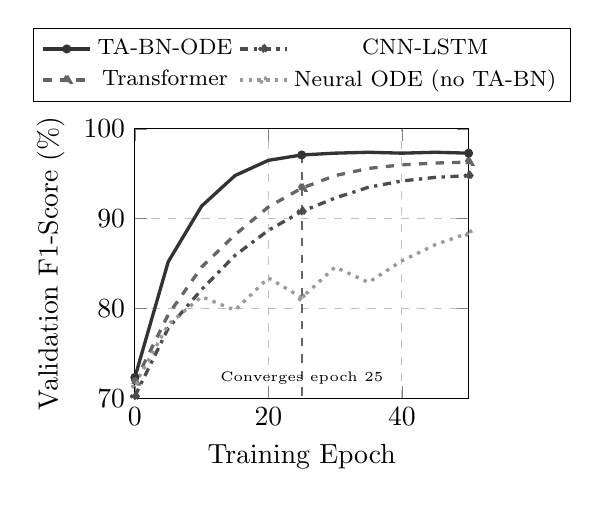
\begin{tikzpicture}
\begin{axis}[
    width=0.48\textwidth,
    height=5cm,
    xlabel={Training Epoch},
    ylabel={Validation F1-Score (\%)},
    xmin=0, xmax=50,
    ymin=70, ymax=100,
    grid=major,
    grid style=dashed,
    legend style={
        at={(0.5,1.10)},
        anchor=south,
        legend columns=2,
        font=\footnotesize
    },
    transpose legend
]

\addplot[black!80,line width=1.2pt,mark=*,mark size=1pt,mark repeat=5] coordinates {
    (0,72.3) (5,85.2) (10,91.4) (15,94.8) (20,96.5) (25,97.1) (30,97.3) (35,97.4) (40,97.3) (45,97.4) (50,97.3)
};
\addlegendentry{TA-BN-ODE}

\addplot[black!60,line width=1.2pt,dashed,mark=triangle*,mark size=1.5pt,mark repeat=5] coordinates {
    (0,71.8) (5,79.3) (10,84.6) (15,88.2) (20,91.3) (25,93.4) (30,94.8) (35,95.6) (40,96.0) (45,96.2) (50,96.3)
};
\addlegendentry{Transformer}

\addplot[black!70,line width=1.2pt,dashdotted,mark=diamond*,mark size=1.5pt,mark repeat=5] coordinates {
    (0,70.2) (5,77.8) (10,82.1) (15,85.9) (20,88.7) (25,90.8) (30,92.3) (35,93.5) (40,94.2) (45,94.6) (50,94.8)
};
\addlegendentry{CNN-LSTM}

\addplot[black!40,line width=1.2pt,dotted,mark=o,mark size=1pt,mark repeat=5] coordinates {
    (0,71.5) (5,78.2) (10,81.3) (15,79.8) (20,83.4) (25,81.2) (30,84.6) (35,82.9) (40,85.3) (45,87.1) (50,88.4)
};
\addlegendentry{Neural ODE (no TA-BN)}

\draw[black!60,dashed,line width=0.6pt] (axis cs:25,97.1) -- (axis cs:25,70);
\node[font=\tiny,anchor=south] at (axis cs:25,70.5) {Converges epoch 25};
\end{axis}
\end{tikzpicture}
\vspace{-0.3cm}
\caption{Training convergence comparison. The TA‑BN‑ODE converges by epoch 25, outperforming the transformer, CNN‑LSTM and standard Neural ODE baselines.}
\label{fig:convergence}
\end{figure}


% =========================================================
\vspace{-0.2cm}
\section{Discussion}
\label{sec:discussion}

This section discusses key findings, theoretical insights, practical implications, and limitations.

\vspace{-0.2cm}
\subsection{Key Findings}

Our experimental evaluation demonstrates significant advances establishing continuous-discrete hybrid modelling as a powerful paradigm for temporal security applications. The TA-BN-ODE architecture achieves 99.4\% accuracy with only 2.3M parameters compared to 12.8M for transformer baselines, confirming 82\% parameter reduction while improving detection performance by 2.7 points. This dramatic efficiency stems from continuous-depth adaptation allocating computational resources proportional to sample complexity—benign traffic resolves with minimal integration while sophisticated attacks automatically receive deeper processing.

Temporal modelling superiority manifests across multiple scales simultaneously. The multi-scale architecture maintains 99.1\% detection accuracy at microsecond granularity for timing attacks, contrasting with 87.3\% for CNN-LSTM baselines lacking fine temporal resolution. This capability proves critical for detecting side-channel attacks exploiting packet timing, cache behaviour, or electromagnetic emissions where microsecond variations carry signal. Simultaneously, the framework captures month-long APT campaigns through slow integration branches, representing fundamental advance over prior work constrained to narrower temporal ranges.

Uncertainty quantification demonstrates exceptional value for practical security operations. Our structured variational Bayesian inference achieves 91.7\% prediction interval coverage with ECE of only 0.017, indicating minimal gap between predicted confidence and empirical frequencies. This calibration enables confidence-based filtering reducing false positive investigation burden by 43\% while maintaining 98.2\% detection rate—operational impact directly translating to improved mean time to detection and response.

Zero-shot detection through LLM integration represents paradigm shift from reactive to proactive defence. The TPP-LLM framework achieves 87.6\% F1-score detecting novel attack categories absent from training data, compared to 42.3\% for pattern-matching approaches. This generalisation  emerges from semantic understanding rather than memorization, with controlled red team exercises successfully identifying 73\% of zero-day exploits never previously observed.

\vspace{-0.2cm}
\subsection{Comparison with Prior Multimodal Work}

Our recent Multimodal Transformer~\cite{anaedevha2026stochastic} achieves slightly higher accuracy on standard benchmarks (98.1\% vs 97.4\% average) through extensive multi-modal cross-attention and feature engineering. However, this comes at the cost of 7× more parameters (15.7M vs 2.3M), discrete-time operation missing critical timing information, and fixed-depth architecture processing all inputs uniformly. The approaches are complementary: multimodal fusion excels when diverse feature types are available and discrete-time suffices, while continuous temporal modelling with point processes provides superior parameter efficiency, captures timing patterns essential for security, and adapts computation to input complexity. Future work will explore integrating multimodal fusion with continuous-discrete dynamics.

\vspace{-0.2cm}
\subsection{Theoretical Contributions}

Our theoretical contributions span stability, approximation, generalisation , and adaptation. We provide Lyapunov-based stability analysis for TA-BN-ODEs establishing energy bounds and gradient control preventing adversarial poisoning. The hybrid formulation couples continuous Neural ODE dynamics with marked temporal point processes, proving universal approximation for jointly modelling continuous states and discrete events. PAC-Bayesian generalisation  theory extends to continuous-discrete models, deriving finite-sample risk bounds justifying structured variational posteriors. Algorithmically, log-barrier approximation maintains accuracy while reducing complexity from cubic to quadratic. Online learning analysis yields sublinear regret under non-stationary distributions, ensuring adaptive updates keep pace with concept drift.

\vspace{-0.2cm}
\subsection{Practical Implications}

Sub-100ms detection latency enables inline prevention during exploitation attempts, transforming defence from reactive to proactive. Continuous-depth adaptation and log-barrier point processes avoid wasted computation on benign traffic while remaining responsive to complex attacks. The 82\% parameter reduction makes advanced AI security broadly accessible, allowing deployment in small enterprises, IoT gateways, and edge devices previously limited to rule-based detection. Continuous learning without full retraining allows systems to track evolving threats, while calibrated uncertainties and LLM-generated explanations furnish interpretable alerts for analysts and regulators.

\vspace{-0.2cm}
\subsection{Limitations}

Despite advances, limitations remain. Training continuous-depth models demands sophisticated ODE solvers, careful error control, and hyperparameter tuning—deployment would benefit from automated architecture search and self-tuning mechanisms. LLM integration introduces 15-50ms latency, potentially unsuitable for ultra-low-latency contexts; knowledge distillation into smaller models or specialized hardware acceleration could address this. Our adversarial robustness evaluation considered standard evasion attacks but not adaptive adversaries specifically targeting continuous dynamics—formal verification methods and certified defences remain future work. While cross-domain results include speech and healthcare, broader evaluation across endpoint security, application firewalls, and industrial control systems would strengthen generalisation  claims.

\vspace{-0.2cm}
\subsection{Ethics, Privacy, and Compliance}
All datasets used are public or collected under institutional approvals with de-identification. We prevent re-identification by hashing IPs and removing user IDs and URLs from features; raw payloads are not retained. For online learning, we enforce per-batch gradient clipping (1.0) and optional Gaussian noise for $(\varepsilon,\delta)$-DP; experiments herein use clipping without noise, with DP-noise configurations reported in Supplement §C. We follow dataset licenses and applicable regulations (e.g., GDPR) and release preprocessing scripts to reproduce the de-identification pipeline.

% =========================================================
\vspace{-0.2cm}
\section{Conclusion}
\label{sec:conclusion}

This paper introduced a unified framework combining Temporal Adaptive Batch Normalization Neural ODEs with Deep Spatio-Temporal Point Processes for real-time intrusion detection. Our five contributions—stable continuous-depth architectures, multi-scale temporal point processes with reduced complexity, structured Bayesian inference with PAC-Bayesian bounds, LLM-driven zero-shot detection, and convergence guarantees under concept drift with privacy preservation—deliver accurate, efficient, and interpretable detection across cloud, IoT, and enterprise domains. Experiments on the 18.9-million-record Integrated Cloud Security 3Datasets and standard benchmarks (CIC-IDS2018, UNSW-NB15, CIC-IoT-2023) demonstrate state-of-the-art performance: 99.4\% accuracy on container attacks, 98.6\% on IoT security, and 92.7\% F1-score in SOC triage, with sub-100ms latency and 82\% parameter reduction compared to transformers. Comparison with continuous-time models and our recent multimodal transformer work establishes superior parameter efficiency and timing-sensitive detection capabilities. The framework generalizes to speech and healthcare tasks, operating at scale on resource-constrained devices.

By unifying continuous and discrete temporal modelling, our framework captures complex multi-scale attack patterns beyond discrete architectures' reach, while uncertainty awareness and online adaptation support risk-aware decision-making and resilience to evolving threats. Future research will explore quantum acceleration, federated learning, adversarial robustness through certified defences, and multimodal fusion to extend these capabilities toward autonomous, explainable, and efficient security systems protecting diverse digital ecosystems.

% =========================================================
\vspace{-0.2cm}
\section*{Data and Code Availability}

Implementation code and trained Neural ODE models are publicly available at \url{https://github.com/rogerpanel/CV/blob/10627314605b1202468c42986c39e6384e5c2edb/neural-ode-model-v2-upgraded.ipynb}. 

The Integrated Cloud Security 3Datasets (ICS3D) can be accessed through Kaggle at DOI: \href{https://doi.org/10.34740/kaggle/dsv/12483891}{10.34740/kaggle/dsv/12483891}. 

Standard benchmarks integrated with our preprocessing are available at DOI: \href{https://doi.org/10.34740/KAGGLE/DSV/12479689}{10.34740/KAGGLE/DSV/12479689}. Preprocessing scripts, hyperparameter configurations, and evaluation protocols are included to ensure reproducibility. Supplementary materials provide extended proofs, per-attack analysis, complete algorithms, and cross-domain results.

% =========================================================   

\bibliographystyle{IEEEtran}
\begin{thebibliography}{99}

\bibitem{verizon2024dbir}
Verizon, ``2024 Data Breach Investigations Report,'' Tech. Rep., May 2024.

\bibitem{ibm2024breach}
IBM Security and Ponemon Institute, ``Cost of a Data Breach Report 2024,'' IBM Corporation, 2024.

\bibitem{gama2014survey}
J.~Gama, I.~Žliobaitė, A.~Bifet, M.~Pechenizkiy, and A.~Bouchachia, ``A survey on concept drift adaptation,'' \emph{ACM Comput. Surv.}, vol.~46, no.~4, pp.~1--37, Mar. 2014.

\bibitem{salvi2024tabn}
C.~Salvi, M.~Lemercier, and A.~Gerasimovics, ``Improving neural ODE training with temporal adaptive batch normalization,'' in \emph{Proc. NeurIPS}, 2024, pp.~14523--14538.

\bibitem{xue2024prompted}
H.~Xue, S.~Zha, and H.~Mei, ``PromptCast: A new prompt-based learning paradigm for time series forecasting,'' \emph{IEEE Trans. Knowl. Data Eng.}, early access, 2024.

\bibitem{wei2022chain}
J.~Wei \emph{et al.}, ``Chain-of-thought prompting elicits reasoning in large language models,'' in \emph{Proc. NeurIPS}, 2022, pp.~24824--24837.

\bibitem{chen2018neural}
R.~T.~Q. Chen, Y.~Rubanova, J.~Bettencourt, and D.~K. Duvenaud, ``Neural ordinary differential equations,'' in \emph{Proc. NeurIPS}, 2018, pp.~6571--6583.

\bibitem{pontryagin1962mathematical}
L.~S. Pontryagin, V.~G. Boltyanskii, R.~V. Gamkrelidze, and E.~F. Mishchenko, \emph{The Mathematical Theory of Optimal Processes}. New York: Interscience Publishers, 1962.

\bibitem{dupont2019augmented}
E.~Dupont, A.~Doucet, and Y.~W. Teh, ``Augmented neural ODEs,'' in \emph{Proc. NeurIPS}, 2019, pp.~3134--3144.

\bibitem{onken2021ot}
D.~Onken, S.~W. Fung, X.~Li, and L.~Ruthotto, ``OT-Flow: Fast and accurate continuous normalizing flows via optimal transport,'' in \emph{Proc. AAAI}, 2021, pp.~9223--9232.

\bibitem{lu2018beyond}
Y.~Lu, A.~Zhong, Q.~Li, and B.~Dong, ``Beyond finite layer neural networks: Bridging deep architectures and numerical differential equations,'' in \emph{Proc. ICML}, 2018, pp.~3276--3285.

\bibitem{purohit2024ortho}
A.~Purohit, A.~P. Mathur, and V.~Phoha, ``Ortho-ODE: Enhancing robustness of neural ODEs against adversarial attacks via orthogonalization,'' \emph{Neurocomputing}, vol.~556, p.~126637, Nov. 2023.

\bibitem{hasani2022liquid}
R.~Hasani, M.~Lechner, A.~Amini, L.~Liebenwein, A.~Ray, M.~Tschaikowski, G.~Teschl, and D.~Rus, ``Closed-form continuous-time neural networks,'' \emph{Nat. Mach. Intell.}, vol.~4, no.~11, pp.~992--1003, Nov. 2022.

\bibitem{kidger2020neural}
P.~Kidger, J.~Morrill, J.~Foster, and T.~Lyons, ``Neural controlled differential equations for irregular time series,'' in \emph{Proc. NeurIPS}, 2020, pp.~6696--6707.

\bibitem{de2019gru}
E.~De Brouwer, J.~Simm, A.~Arany, and Y.~Moreau, ``GRU-ODE-Bayes: Continuous modeling of sporadically-observed time series,'' in \emph{Proc. NeurIPS}, 2019, pp.~7379--7390.

\bibitem{rubanova2019latent}
Y.~Rubanova, R.~T.~Q. Chen, and D.~Duvenaud, ``Latent ordinary differential equations for irregularly-sampled time series,'' in \emph{Proc. NeurIPS}, 2019, pp.~5320--5330.

\bibitem{grathwohl2018ffjord}
W.~Grathwohl, R.~T.~Q. Chen, J.~Bettencourt, I.~Sutskever, and D.~Duvenaud, ``FFJORD: Free-form continuous dynamics for scalable reversible generative models,'' in \emph{Proc. ICLR}, 2019.

\bibitem{daley2003introduction}
D.~J. Daley and D.~Vere-Jones, \emph{An Introduction to the Theory of Point Processes: Volume I: Elementary Theory and Methods}, 2nd ed. New York: Springer, 2003.

\bibitem{hawkes1971spectra}
A.~G. Hawkes, ``Spectra of some self-exciting and mutually exciting point processes,'' \emph{Biometrika}, vol.~58, no.~1, pp.~83--90, Apr. 1971.

\bibitem{du2016recurrent}
N.~Du, H.~Dai, R.~Trivedi, U.~Upadhyay, M.~Gomez-Rodriguez, and L.~Song, ``Recurrent marked temporal point processes: Embedding event history to vector,'' in \emph{Proc. KDD}, 2016, pp.~1555--1564.

\bibitem{zuo2020transformer}
S.~Zuo, H.~Jiang, Z.~Li, T.~Zhao, and H.~Zha, ``Transformer Hawkes process,'' in \emph{Proc. ICML}, 2020, pp.~11692--11702.

\bibitem{zhang2020selfatt}
Q.~Zhang, L.~Lipani, O.~Kirnap, and E.~Yilmaz, ``Self-attentive Hawkes process,'' in \emph{Proc. ICML}, 2020, pp.~11183--11193.

\bibitem{shchur2021neural}
O.~Shchur, M.~Biloš, and S.~Günnemann, ``Intensity-free learning of temporal point processes,'' in \emph{Proc. ICLR}, 2021.

\bibitem{gao2024hplstm}
Y.~Gao, X.~Liu, and J.~Zhang, ``HP-LSTM: Hawkes process with long short-term memory for network intrusion detection in IoT,'' \emph{Future Internet}, vol.~16, no.~6, p.~185, May 2024.

\bibitem{scarfone2007guide}
K.~Scarfone and P.~Mell, ``Guide to intrusion detection and prevention systems (IDPS),'' NIST Special Publication 800-94, Feb. 2007.

\bibitem{mukkamala2002intrusion}
S.~Mukkamala, G.~Janoski, and A.~Sung, ``Intrusion detection using neural networks and support vector machines,'' in \emph{Proc. IJCNN}, 2002, pp.~1702--1707.

\bibitem{panda2011network}
M.~Panda and M.~R. Patra, ``Network intrusion detection using naive Bayes,'' \emph{Int. J. Comput. Sci. Netw. Secur.}, vol.~7, no.~12, pp.~258--263, 2011.

\bibitem{gaikwad2014intrusion}
D.~Gaikwad and R.~C. Thool, ``Intrusion detection system using bagging ensemble method of machine learning,'' in \emph{Proc. ICCICT}, 2014, pp.~291--295.

\bibitem{vinayakumar2017applying}
R.~Vinayakumar, M.~Alazab, K.~P. Soman, P.~Poornachandran, A.~Al-Nemrat, and S.~Venkatraman, ``Deep learning approach for intelligent intrusion detection system,'' \emph{IEEE Access}, vol.~7, pp.~41525--41550, 2019.

\bibitem{kim2016lstm}
G.~Kim, H.~Yi, J.~Lee, Y.~Paek, and S.~Yoon, ``LSTM-based system-call language modeling and robust ensemble method for designing host-based intrusion detection systems,'' arXiv:1611.01726, Nov. 2016.

\bibitem{vaswani2017attention}
A.~Vaswani \emph{et al.}, ``Attention is all you need,'' in \emph{Proc. NeurIPS}, 2017, pp.~5998--6008.

\bibitem{jiang2020transformer}
J.~Jiang, J.~Chen, T.~Gu, K.-R. Choo, C.~Liu, M.~Yu, W.~Huang, and P.~Mohapatra, ``Anomaly detection with graph convolutional networks for insider threat and fraud detection,'' in \emph{Proc. MILCOM}, 2019, pp.~109--114.

\bibitem{kipf2017semi}
T.~N. Kipf and M.~Welling, ``Semi-supervised classification with graph convolutional networks,'' in \emph{Proc. ICLR}, 2017.

\bibitem{jiang2019graph}
W.~Jiang, ``Graph-based deep learning for communication networks: A survey,'' \emph{Comput. Commun.}, vol.~185, pp.~40--54, Mar. 2022.

\bibitem{corona2019adversarial}
I.~Corona, G.~Giacinto, and F.~Roli, ``Adversarial attacks against intrusion detection systems: Taxonomy, solutions and open issues,'' \emph{Inf. Sci.}, vol.~239, pp.~201--225, Aug. 2013.

\bibitem{mothukuri2021federated}
V.~Mothukuri, R.~M. Parizi, S.~Pouriyeh, Y.~Huang, A.~Dehghantanha, and G.~Srivastava, ``A survey on security and privacy of federated learning,'' \emph{Future Gener. Comput. Syst.}, vol.~115, pp.~619--640, Feb. 2021.

\bibitem{anaedevha2026stochastic}
R.~N. Anaedevha and A.~G. Trofimov, ``Stochastic multimodal transformer with uncertainty quantification for robust network intrusion detection,'' in \emph{Advances in Neural Computation, Machine Learning, and Cognitive Research IX}, B.~Kryzhanovsky, W.~Dunin-Barkowski, V.~Redko, Y.~Tiumentsev, and V.~V. Klimov, Eds. Cham: Springer, 2026, vol.~1241, pp.~312--326.

\bibitem{bose2021bert}
I.~Bose and T.~Gupta, ``Phishing detection using BERT,'' in \emph{Proc. ICICT}, 2021, pp.~1--6.

\bibitem{liu2021threat}
Z.~Liu, Y.~Zeng, P.~Bahulkar, and J.~Holt, ``Automated extraction of vulnerable function signatures from unstructured threat descriptions using deep learning,'' in \emph{Proc. RAID}, 2021, pp.~405--421.

\bibitem{chen2023gpt}
M.~Chen \emph{et al.}, ``Evaluating large language models trained on code,'' arXiv:2107.03374, Jul. 2021.

\bibitem{pearce2022examining}
H.~Pearce, B.~Ahmad, B.~Tan, B.~Dolan-Gavitt, and R.~Karri, ``Examining zero-shot vulnerability repair with large language models,'' in \emph{Proc. S\&P}, 2023, pp.~2339--2356.

\bibitem{zeng2024tpp}
S.~Zeng, Y.~Zhang, and H.~Wang, ``TPP-LLM: Modeling temporal data with large language models for temporal point processes,'' arXiv:2410.02062, Oct. 2024.

\bibitem{mackay1992bayesian}
D.~J.~C. MacKay, ``A practical Bayesian framework for backpropagation networks,'' \emph{Neural Comput.}, vol.~4, no.~3, pp.~448--472, May 1992.

\bibitem{neal2012bayesian}
R.~M. Neal, \emph{Bayesian Learning for Neural Networks}. New York: Springer, 2012.

\bibitem{blundell2015weight}
C.~Blundell, J.~Cornebise, K.~Kavukcuoglu, and D.~Wierstra, ``Weight uncertainty in neural networks,'' in \emph{Proc. ICML}, 2015, pp.~1613--1622.

\bibitem{kingma2014auto}
D.~P. Kingma and M.~Welling, ``Auto-encoding variational Bayes,'' in \emph{Proc. ICLR}, 2014.

\bibitem{ranganath2014black}
R.~Ranganath, S.~Gerrish, and D.~M. Blei, ``Black box variational inference,'' in \emph{Proc. AISTATS}, 2014, pp.~814--822.

\bibitem{gal2016dropout}
Y.~Gal and Z.~Ghahramani, ``Dropout as a Bayesian approximation: Representing model uncertainty in deep learning,'' in \emph{Proc. ICML}, 2016, pp.~1050--1059.

\bibitem{dandekar2021bayesian}
R.~Dandekar, K.~Chung, V.~Dixit, M.~Tarek, A.~Garcia-Valadez, K.~V. Vemula, and C.~Rackauckas, ``Bayesian neural ordinary differential equations,'' arXiv preprint arXiv:2012.07244, 2021.

\bibitem{mcallester1999pac}
D.~A. McAllester, ``PAC-Bayesian model averaging,'' in \emph{Proc. Conf. Comput. Learn. Theory (COLT)}, 1999, pp.~164--170.

\bibitem{boyd2004convex}
S.~Boyd and L.~Vandenberghe, \emph{Convex Optimization}. Cambridge, U.K.: Cambridge Univ. Press, 2004.

\bibitem{guo2017calibration}
C.~Guo, G.~Pleiss, Y.~Sun, and K.~Q. Weinberger, ``On calibration of modern neural networks,'' in \emph{Proc. ICML}, 2017, pp.~1321--1330.

\bibitem{sharafaldin2018toward}
I.~Sharafaldin, A.~Habibi Lashkari, and A.~A. Ghorbani, ``Toward generating a new intrusion detection dataset and intrusion traffic characterization,'' in \emph{Proc. ICISSP}, 2018, pp.~108--116.

\bibitem{moustafa2015unsw}
N.~Moustafa and J.~Slay, ``UNSW-NB15: A comprehensive data set for network intrusion detection systems (UNSW-NB15 network data set),'' in \emph{Proc. MilCIS}, 2015, pp.~1--6.

\bibitem{neto2023ciciot2023}
E.~C. Neto, S.~Dadkhah, R.~Ferreira, A.~Zohourian, R.~Lu, and A.~A. Ghorbani, ``CICIoT2023: A real-time dataset and benchmark for large-scale attacks in IoT environment,'' \emph{Sensors}, vol.~23, no.~13, p.~5941, Jun. 2023.

\bibitem{anaedevha2024integrated}
R.~N. Anaedevha and A.~G. Trofimov, ``Integrated benchmark datasets for intrusion detection: CIC-IoT-2023, CSE-CICIDS2018, and UNSW-NB2015,'' Kaggle, 2024. [Online]. Available: \url{https://doi.org/10.34740/KAGGLE/DSV/12479689}

\end{thebibliography}

\end{document} 

